\documentclass[11pt,reqno]{amsart}
\usepackage[T1]{fontenc}
\usepackage{lmodern,amsmath,amssymb,mathtools,microtype}
\usepackage[a4paper,margin=28mm]{geometry}
\usepackage{xcolor,booktabs,enumitem,needspace}
\usepackage{tikz}
\usetikzlibrary{arrows.meta,positioning,calc}
\definecolor{linkteal}{RGB}{0,83,91}
\usepackage[colorlinks=true,linkcolor=linkteal,citecolor=linkteal,urlcolor=linkteal]{hyperref}
\usepackage[nameinlink,noabbrev]{cleveref}
\hypersetup{pdftitle={Greatest Quantum Channels with Prescribed Maximal Information},pdfauthor={Harjas Sandhu},pdfsubject={Complete RLD profiles, channel comparison, and injective von Neumann algebras},pdfkeywords={quantum channel, RLD Fisher information, maximal f-divergence, injectivity, deficiency}}
\newtheorem{theorem}{Theorem}[section]
\newtheorem{proposition}[theorem]{Proposition}
\newtheorem{lemma}[theorem]{Lemma}
\newtheorem{corollary}[theorem]{Corollary}
\theoremstyle{definition}
\newtheorem{definition}[theorem]{Definition}
\newtheorem{example}[theorem]{Example}
\theoremstyle{remark}
\newtheorem{remark}[theorem]{Remark}
\numberwithin{equation}{section}
\DeclareMathOperator{\Tr}{Tr}
\DeclareMathOperator{\id}{id}
\DeclareMathOperator{\Rea}{Re}
\DeclareMathOperator{\Ima}{Im}
\DeclareMathOperator{\supp}{supp}
\DeclareMathOperator{\diag}{diag}
\DeclareMathOperator{\spanop}{span}
\DeclareMathOperator{\dist}{dist}
\newcommand{\M}{\mathcal M}
\newcommand{\A}{\mathcal A}
\newcommand{\C}{\mathcal C}
\newcommand{\HH}{\mathcal H}
\newcommand{\tr}{\operatorname{tr}}
\newcommand{\Sone}{\mathcal S_1}
\newcommand{\B}{\mathcal B}
\newcommand{\E}{\mathsf E}
\newcommand{\F}{\mathsf F}
\newcommand{\G}{\mathsf G}
\newcommand{\R}{\mathsf R}
\newcommand{\one}{\mathbf 1}
\newcommand{\norm}[1]{\left\lVert#1\right\rVert}
\newcommand{\abs}[1]{\left\lvert#1\right\rvert}
\newcommand{\ip}[2]{\left\langle#1,#2\right\rangle}
\newcommand{\dd}{\mathrm d}
\newcommand{\ee}{\mathrm e}
\newcommand{\ii}{\mathrm i}
\newcommand{\defic}{\delta}
\newcommand{\rld}{\mathfrak g}
\newcommand{\maxdiv}{\widehat D}
\newcommand{\cut}[2]{\one_{(#1,\infty)}(#2)}
\setlist[enumerate]{label=\textup{(\roman*)},leftmargin=2em,itemsep=3pt}
\setlength{\emergencystretch}{2em}
\allowdisplaybreaks[2]
\title[Greatest channels with prescribed maximal information]{Greatest Quantum Channels\\with Prescribed Maximal Information}
\author{Harjas Sandhu}
\address{The University of Queensland}
\email{harjas.sandhu@student.uq.edu.au}
\date{6 November 2026}
\subjclass[2020]{Primary 81P45; Secondary 46L10, 46L60, 62B05, 68Q25}
\keywords{Quantum channel comparison, RLD Fisher information, maximal divergence, injective von Neumann algebra, statistical deficiency}
\begin{document}
\raggedbottom
\begin{abstract}
Equality of quantum information measures need not imply recoverability. We study the class of all channels having the same right logarithmic derivative Fisher information for every faithful input, tangent, and finite reference system. These data determine a generated von Neumann algebra, its labelled normalized channel, and a faithful normal state. For finite outputs this invariant yields a greatest channel under deterministic postprocessing, of minimum possible output dimension. For separable trace-class outputs and a tracial invariant state, a greatest member exists exactly when the invariant is a countable product of finite matrix algebras. Arbitrarily accurate greatest members inside the same exact profile class exist exactly when the invariant is injective. In the latter statement a common sequence approximating each fixed target already implies the existence of a uniformly approximating sequence. The proofs combine physical resolvent tests, spectral pinching, finite-dimensional averaging, and established operator-algebraic approximation theory. We give an explicit free-group obstruction, polynomial-bit separating tests for rational finite channels, and a fixed full-support family for which the optimized capacity of the profile class is discontinuous although every physical channel is antidegradable. The atomic/injective distinction and the underlying sufficiency and amenability machinery are established; the formulation here fixes the complete information profile and requires its optimizing sources to remain in that class.
\end{abstract}
\maketitle
\setcounter{tocdepth}{1}
\tableofcontents
\clearpage

% Included source: sections/01-introduction
\section{Introduction}

How much of a quantum channel is determined by all its local information geometry? Even when a metric is evaluated at every input, information equality can identify channels with different abilities to distinguish states or transmit quantum data. A sharper question is therefore to fix the entire information profile and ask which physical realizations it permits. Is one realization at least as informative as every other, in the operational sense that all the others can be obtained from it by a channel?

We answer this question for complete right logarithmic derivative (RLD) profiles. Here \emph{complete} means that an arbitrary finite reference system may be retained: the channel acts on one part of an entangled input, while the reference is untouched. Equality is required for every faithful input state and every physical tangent. The same equivalence relation results from equality of all complete maximal $f$-divergences. Neither condition is ordinary statistical equivalence.

The invariant behind these profiles is particularly concrete. For a channel $\E$ with finite input, set $\Omega=\E(I)$ and remove the two outer factors $\Omega^{1/2}$:
\[
 \E(X)=\Omega^{1/2}T(X)\Omega^{1/2},\qquad T(I)=I.
\]
The normalized outputs $T(X)$ generate an algebra $\M$. The density $\Omega$ supplies the state $\tau(Z)=\Tr(\Omega Z)/a$, where $a$ is the input dimension. The complete profile remembers the triple $(\M,T,\tau)$, including the labels $X\mapsto T(X)$; it forgets how that triple is represented inside a particular output Hilbert space.

For finite-dimensional outputs, this description produces a greatest representative: represent each simple matrix block once, and put its prescribed state back around the normalized map. Every other representative is obtained by a trace-preserving preparation map. This representative also has the smallest possible output dimension. A smallest-dimensional representative need not itself be greatest; a two-state example in \cref{ex:two-pure} makes that distinction explicit.

For infinite outputs the category of physical output systems matters. We require ordinary density operators on separable Hilbert spaces and normal physical postprocessings. If $\tau$ is tracial, an exact greatest member exists precisely for countable products of finite matrix blocks. If $\M$ is diffuse and injective, exact greatestness fails, but arbitrary uniform accuracy is possible without leaving the exact profile class. If $\M$ is noninjective, even one sequence of sources approximating every fixed target is impossible. The approximation norm is the diamond norm, including arbitrary references at the comparison stage.

The restriction to a tracial $\tau$ is essential to the proofs given here. The finite-dimensional classification and greatest-representative theorem do not require it. The infinite nontracial problem remains open in this paper.

\subsection{Predecessors and the precise comparison problem}

Maximal divergences and reverse tests already provide much of the relevant geometry. Matsumoto's spectral reverse test \cite[Theorem~6.1]{Matsumoto} and Hiai's von Neumann algebraic formulation \cite[Lemma~6.1 and Theorem~6.3]{Hiai} explain why a noncommutative experiment can have a classical maximal-divergence realization. Hiai and Mosonyi \cite[Theorem~3.34 and Example~4.8]{HiaiMosonyi} distinguish maximal-divergence equality from ordinary reversibility. We use this distinction throughout. The elementary example in \cref{ex:two-pure} is a channel-level manifestation of it.

Canonical sufficient quantum experiments have an extensive theory. Gu\c t\u a and Jen\v cov\'a \cite[Corollary~3.4 and Theorem~3.5]{GutaJencova} use canonical states and Connes cocycles; Kuramochi \cite[Theorem~1 and Corollary~2]{KuramochiMinimal} proves existence and uniqueness of minimal sufficient experiments. Those results concern ordinary statistical equivalence. Here an exact maximal-information class can contain statistically inequivalent members, and the object sought is a \emph{greatest} member of that larger class. The transpose-channel formula in \cref{prop:concrete-lift} uses the established Petz reconstruction mechanism, rather than a new recovery formalism. Related whitening and recovery structures appear in \cite[Theorem~5.7]{BSMarkov}.

The underlying distinction between atomic exact realization and injective approximate realization is also established. St\o rmer's projection theorem \cite[p.~47]{Stormer}, Holevo's discussion of continuous classical outputs \cite[\S1]{Holevo}, and Kuramochi's discrete-outcome realization criterion \cite[Lemma~6 and Theorem~5]{KuramochiMinimal} exhibit the normality obstruction. Most closely, Okamura and Ozawa \cite[Theorem~IV.4 and the paragraph following it]{OkamuraOzawa} identify atomicity and injectivity with exact and approximate extension properties for instruments whose extensions range in the original algebra. Their approximation rests on Anantharaman-Delaroche's normal completely positive approximation theorem \cite[Corollary~3.9]{AD}. These results already give an operational atomic/injective distinction.

Our formulation imposes additional, explicit requirements: all sources must have one prescribed \emph{complete} maximal-information profile; one source must work for every realization of that profile; and the approximation must hold in diamond norm. The two bridges needed for these requirements are spectral pinching, which turns postprocessing performance into near-centrality, and finite-dimensional Haar averaging, which keeps the sources inside the exact class. The conversion of near-central states into injectivity is standard amenability machinery; compare \cite[Theorems~3.1.6 and 3.2.2]{Brown}. The implication from injectivity to finite-dimensional approximation is Connes' theorem \cite[Chapter~V, \S7, Theorem~6]{Connes}.

General quantum comparison theorems are complementary. Jen\v cov\'a's diamond-deficiency theorem \cite[Theorem~1]{JencovaComparison} characterizes the quality of postprocessing an already specified source. Ganesan, Gao, Pandey, and Plosker \cite[Theorems~3.5, 3.13, and 3.18]{Ganesan} characterize injectivity and majorization using conditional min-entropy and tensor norms. In the latter comparison the physical output algebra $\B(\HH)$ is injective even when the normalized invariant $\M\subset\B(\HH)$ is not. Thus these theorems do not by themselves choose a source in a prescribed profile class. Jen\v cov\'a's trace-norm criterion \cite[Theorem~4]{JencovaRecovery} concerns sufficiency of an existing map on a pair of states. Our pinching argument instead compares different realizations of the same normalized channel.

Finally, RLD must be distinguished from symmetric logarithmic derivative (SLD) geometry. Complete SLD, Umegaki, and Holevo comparison problems, including the undecidability results of \cite{CompleteOrders}, use different metrics or different comparison quantifiers. The polynomial algorithm for \emph{exact RLD-profile equality} proved here does not decide those order problems.

\clearpage
\subsection{A conceptual overview}

The proof has two directions. The first extracts an algebra from physical tests. A reference system is arranged as a path. Successive edges carry successive normalized outputs, so the first nonzero endpoint coefficient of a resolvent is an ordered product. Four elementary reference projectors read its real and imaginary parts. All physical tests therefore determine all ordered moments, and faithfulness reconstructs the labelled algebra.

The second direction realizes that algebra as efficiently as the output category allows. A finite algebra can be represented block by block without multiplicities. An atomic infinite algebra admits the corresponding countable direct sum. For a diffuse algebra, concentrating a trace-class density on finer spectral cuts prevents a single greatest density-operator realization. Injectivity nevertheless supplies finite subalgebras. Averaging the density over each finite unitary group produces sources with \emph{exactly} the original profile, while their finite quotients simulate every target uniformly.

\begin{figure}[!ht]
\centering
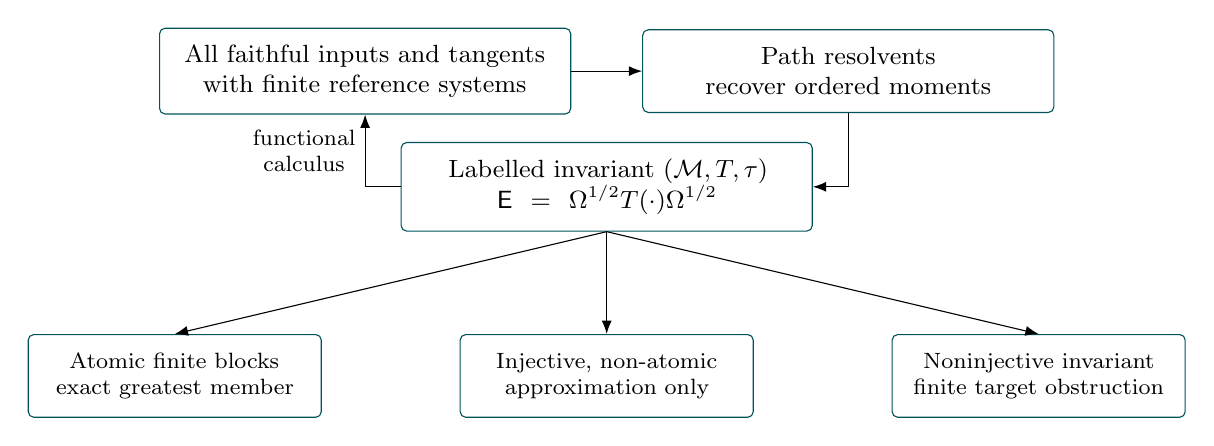
\begin{tikzpicture}[>=Latex,font=\small,
 box/.style={draw=linkteal,rounded corners=2pt,align=center,text width=4.8cm,minimum height=1.05cm,inner sep=6pt},
 note/.style={align=center,font=\footnotesize}]
 \node[box] (tests) {All faithful inputs and tangents\\with finite reference systems};
 \node[box,right=9mm of tests] (moments) {Path resolvents\\recover ordered moments};
 \node[box,below=9mm of $(tests)!0.5!(moments)$] (triple) {Labelled invariant $(\M,T,\tau)$\\$\E=\Omega^{1/2}T(\cdot)\Omega^{1/2}$};
 \draw[->] (tests)--(moments);
 \draw[->] (moments.south) |- (triple.east);
 \draw[->] (triple.west) -| node[pos=.75,left,note]{functional\\calculus} (tests.south);
 \node[box,font=\footnotesize,text width=3.3cm,below left=13mm and 10mm of triple] (atomic) {Atomic finite blocks\\exact greatest member};
 \node[box,font=\footnotesize,text width=3.3cm,below=13mm of triple] (injective) {Injective, non-atomic\\approximation only};
 \node[box,font=\footnotesize,text width=3.3cm,below right=13mm and 10mm of triple] (noninj) {Noninjective invariant\\finite target obstruction};
 \draw[->] (triple.south)--(atomic.north);
 \draw[->] (triple.south)--(injective.north);
 \draw[->] (triple.south)--(noninj.north);
\end{tikzpicture}
\caption{The information profile determines an algebraic realization problem. The lower row classifies tracial invariants; ``atomic finite blocks'' means a countable product of finite matrix algebras. Approximation uses sources inside the exact class and is uniform over all targets. The finite-dimensional theorem also allows nontracial states.}
\label{fig:overview}
\end{figure}

Conversely, suppose one sequence simulates every fixed realization. Spectral pinching gives fixed targets attaining the largest possible binary testing norm for each normalized generator and threshold. Small testing deficits force the source densities to almost commute with those spectral projections. A limiting central state then produces a completely positive projection onto $\M$, proving injectivity. This limiting projection may be nonnormal; the physical converters used throughout are normal.

\subsection{Organization and scope}

\Cref{sec:framework} states the classification and realization theorems. \Cref{sec:profile,sec:finite} prove the finite theory and the profile invariant. \Cref{sec:exact,sec:approximate} prove the tracial infinite-output criteria. Explicit diffuse and free-group examples appear in \cref{sec:examples}. \Cref{sec:stability} separates exact symbolic identification from unstable optimization over a profile class. The appendices contain witness bounds, a finite free-group obstruction, a rational full-support instability certificate, and applications of established identification and semialgebraic machinery. No effectiveness claim is made for the infinite-dimensional filtration or its convergence rate.


\clearpage

% Included source: sections/02-framework
\section{Profiles, realizations, and the main theorems}\label{sec:framework}

\subsection{Channels and physical profiles}

Write $M_a=\B(\mathbb C^a)$ and let $\Sone(\HH)$ denote the trace-class operators on a separable Hilbert space. A channel is a completely positive trace-preserving map
\[
 \E:M_a\longrightarrow\Sone(\HH).
\]
All traces below are unnormalized unless a subscript indicates otherwise. We remove the kernel of $\Omega_\E=\E(I_a)$ from $\HH$. This is the \emph{effective output space}; on it $\Omega_\E$ is faithful and $\Tr\Omega_\E=a$. It need not have a bounded inverse.

There is a unique bounded unital completely positive map $T_\E:M_a\to\B(\HH)$ such that
\begin{equation}\label{eq:normalization}
 \E(X)=\Omega_\E^{1/2}T_\E(X)\Omega_\E^{1/2}.
\end{equation}
We prove this assertion in \cref{lem:bounded-normalization}. Define
\begin{equation}\label{eq:invariant}
 \M_\E=W^*(T_\E(M_a)),\qquad
 \tau_\E(Z)=\frac1a\Tr(\Omega_\E Z).
\end{equation}
The state $\tau_\E$ is faithful and normal. In general it is not a trace. Trace preservation says exactly
\begin{equation}\label{eq:trace-label}
 a\tau_\E(T_\E(X))=\Tr X.
\end{equation}

Here $W^*$ means the weakly closed unital $*$-algebra generated by the indicated operators. It includes limits of bounded polynomial approximants, not only finite polynomials. A normal map preserves bounded increasing limits of positive operators. The labels $X\mapsto T_\E(X)$ retain which input produced each generator, and $\tau_\E$ records their weighted expectations.

For a reference $\mathbb C^r$ put $\E_r=\E\otimes\id_r$ and $T_r=T_\E\otimes\id_r$. A faithful density $\rho\in M_a\otimes M_r$ has trace one, and a physical tangent is $K=K^*$ with $\Tr K=0$. Set
\begin{equation}\label{eq:rld}
 \rld_\E(\rho,K)
 =\Tr\!\left[(\Omega_\E\otimes I_r)
 T_r(K)T_r(\rho)^{-1}T_r(K)\right].
\end{equation}
This expression is finite: $T_r(\rho)\ge\lambda_{\min}(\rho)I$. For finite outputs it equals the usual RLD quadratic form
\[
 \Tr\bigl[\E_r(K)\E_r(\rho)^{-1}\E_r(K)\bigr]
\]
on the effective support. Formula \eqref{eq:rld} gives its closed quadratic-form interpretation in infinite dimensions. There is no assumption that $\E_r(\rho)^{-1}$ is bounded.

The tangent $K$ describes the infinitesimal displacement along $\rho+sK$. Faithfulness of $\rho$ ensures that this is a state for sufficiently small $s$ of either sign. The quadratic form measures this displacement after the channel. Requiring every reference system makes these tests sensitive to the order of the normalized output operators.

\begin{definition}
Channels $\E$ and $\F$ with the same input are \emph{profile equivalent}, written $\E\sim\F$, if
\[
 \rld_\E(\rho,K)=\rld_\F(\rho,K)
\]
for every finite $r$, faithful density $\rho$, and traceless Hermitian $K$. The \emph{profile class} $\C(\E)$ consists of all such $\F$ with separable effective output spaces.
\end{definition}

For completeness, the corresponding maximal $f$-profile has a bounded description. Let $f:(0,\infty)\to\mathbb R$ be operator convex with $f(1)=0$, and let $\alpha,\beta$ be faithful input densities, possibly with a reference. With $S=T_r(\beta)$ and $A=T_r(\alpha)$, it is
\begin{equation}\label{eq:maxf}
 \maxdiv_f(\E_r(\alpha)\Vert\E_r(\beta))
 =\Tr\!\left[(\Omega_\E\otimes I_r)
 S^{1/2}f(S^{-1/2}AS^{-1/2})S^{1/2}\right].
\end{equation}
Both $A$ and $S$ are bounded above and bounded away from zero. This is the usual maximal divergence, with the same support convention. It includes the maximal quadratic divergence $f_2(x)=(x-1)^2$.

\subsection{Deterministic comparison}

A physical postprocessing $\R:\Sone(\HH_1)\to\Sone(\HH_2)$ is completely positive and trace preserving. Its adjoint on bounded operators is normal and unital. We write $\G\succeq\F$ if $\F=\R\G$ for such an $\R$, and define
\begin{equation}\label{eq:deficiency}
 \defic(\G,\F)=\inf_\R\norm{\F-\R\G}_\diamond.
\end{equation}
The diamond norm is the supremum of the trace norm over finite references and trace-norm-one inputs. For a finite-dimensional input the reference dimension can be restricted to $a$. The orientation in \eqref{eq:deficiency} is fixed: the first argument is the available source, the second the desired target.

A \emph{greatest member} $\Gamma$ of a profile class belongs to the class and satisfies $\Gamma\succeq\F$ for every member $\F$. It is stronger than merely being maximal. Two greatest members necessarily simulate one another.

\begin{theorem}[The complete profile invariant]\label{thm:classification}
For channels with finite common input and separable effective outputs, the following are equivalent:
\begin{enumerate}
 \item $\E\sim\F$.
 \item All finite-reference maximal $f$-profiles agree for faithful input pairs and all operator-convex $f$ with $f(1)=0$.
 \item There is a normal $*$-isomorphism $\theta:\M_\E\to\M_\F$ satisfying
 \[
  \theta(T_\E(X))=T_\F(X),\qquad
  \tau_\F\circ\theta=\tau_\E.
 \]
\end{enumerate}
No traciality assumption is required. The same invariant also determines the profiles of every finite tensor power.
\end{theorem}

The isomorphism preserves the input labels; an abstract isomorphism of $\M_\E$ and $\M_\F$ is insufficient. In view of this theorem we may fix an abstract invariant $(\M,T,\tau)$. Its realizations are exactly
\begin{equation}\label{eq:all-realizations}
 \F(X)=\Omega_\F^{1/2}\pi_\F(T(X))\Omega_\F^{1/2},\qquad
 \Tr[\Omega_\F\pi_\F(Z)]=a\tau(Z),
\end{equation}
where $\pi_\F$ is a faithful normal representation on a separable Hilbert space and $\Omega_\F$ is faithful trace class. We consider invariants arising from at least one channel, so this class is nonempty.

\begin{theorem}[Finite invariant: a smallest greatest member]\label{thm:finite}
Suppose $\M=\bigoplus_{j=1}^sM_{n_j}$. In its multiplicity-one representation let $h=\bigoplus_jh_j>0$ be the density of $a\tau$ relative to the ordinary matrix trace. Then
\begin{equation}\label{eq:finite-canonical}
 \Gamma(X)=h^{1/2}T(X)h^{1/2}
\end{equation}
is a greatest member of the full separable-output profile class. Its output dimension $\sum_jn_j$ is the minimum possible effective output dimension in the class. The state $\tau$ may be nontracial.
\end{theorem}

The next two theorems impose traciality. A finite von Neumann algebra with a faithful normal trace is \emph{injective} if, in a faithful representation, it is the range of a unital completely positive projection from the ambient bounded operators. The projection need not be normal. Injectivity is representation independent. In our separable setting Connes' theorem identifies it with hyperfiniteness, that is, weak density of an increasing sequence of finite-dimensional subalgebras.

\Needspace{16\baselineskip}
\begin{theorem}[Exact greatest realization in the tracial case]\label{thm:exact}
Let $(\M,T,\tau)$ arise from a channel with finite input and separable effective output, and assume that $\tau$ is tracial. Its profile class has a greatest member if and only if
\begin{equation}\label{eq:atomic}
 \M\cong\prod_{j\in J}M_{n_j},\qquad |J|\le\aleph_0,\quad n_j<\infty.
\end{equation}
If $\tau=\sum_jp_j\tr_{n_j}$, where $p_j>0$ and $\sum_jp_j=1$, a greatest member is
\begin{equation}\label{eq:atomic-channel}
 \Gamma(X)=\bigoplus_{j\in J}\frac{ap_j}{n_j}T_j(X).
\end{equation}
The algebra in \eqref{eq:atomic} is a bounded von Neumann product; the output in \eqref{eq:atomic-channel} is a trace-norm summable direct sum.
\end{theorem}

\begin{theorem}[Approximate greatest realization in the tracial case]\label{thm:approximate}
Under the assumptions of \cref{thm:exact}, the following are equivalent:
\begin{enumerate}
 \item For every $\varepsilon>0$ there is a single $\G\in\C$ with
 $\sup_{\F\in\C}\defic(\G,\F)<\varepsilon$.
 \item There is a single sequence $(\G_k)\subset\C$ such that
 $\defic(\G_k,\F)\to0$ for every fixed $\F\in\C$.
 \item $\M$ is injective, equivalently hyperfinite.
\end{enumerate}
If these conditions hold, a sequence can be chosen with uniform error tending to zero. The sequence in \textup{(ii)} need not itself converge uniformly. Its outputs may be infinite dimensional, and the decoder may depend on the source and the target. No computable filtration or convergence modulus is asserted.
\end{theorem}

\begin{corollary}[Finite obstruction]\label{cor:finite-obstruction}
If $\M$ is noninjective, there are finitely many fixed class members $\F_1,\ldots,\F_\ell$ and $\eta>0$ such that
\[
 \max_{1\le j\le\ell}\defic(\G,\F_j)\ge\eta
 \quad\text{for every }\G\in\C.
\]
\end{corollary}

These results distinguish exact realization, approximate realization, and effective construction. For example, a diffuse commutative invariant is injective and admits arbitrarily accurate greatest members, but no exact greatest member. The free-group example in \cref{prop:free-group} has neither property. None of these alternatives by itself supplies an algorithm for constructing an infinite-dimensional approximation from a black box.



% Included source: sections/03-profile
\section{Recovering the labelled algebra from physical tests}\label{sec:profile}

The main issue is order. A scalar trace of a polynomial may discard the order of its factors, and a transpose preserves every unreferenced maximal divergence. A reference path records an ordered product before taking the state. This section makes that observation precise and proves \cref{thm:classification}.

\subsection{Bounded normalization}

\begin{lemma}\label{lem:bounded-normalization}
Equation \eqref{eq:normalization} defines a unique bounded UCP map on the effective output space. The state in \eqref{eq:invariant} is faithful and normal, and \eqref{eq:rld} and \eqref{eq:maxf} agree with their usual output-space definitions.
\end{lemma}

\begin{proof}
For $0\le X\le cI$, complete positivity gives $0\le\E(X)\le c\Omega$. On the dense range of $\Omega^{1/2}$ define the quadratic form
\[
 \ip{\Omega^{1/2}\xi}{T(X)\Omega^{1/2}\eta}
 =\ip{\xi}{\E(X)\eta}.
\]
The domination makes this a bounded positive form of norm at most $c$. Extend linearly from positive matrices. The same argument applied to positive matrices over $M_a$ proves complete positivity, and $T(I)=I$. Density proves uniqueness. Faithfulness of $\tau$ follows because $\Tr\Omega Z=0$ for $Z\ge0$ implies $Z^{1/2}\Omega^{1/2}=0$, hence $Z=0$; normality is immediate from the trace-class density.

Here is also why compact densities cause no inverse problem in the profiles. Write $W=\Omega\otimes I_r$, $S=T_r(\rho)>0$, $D=T_r(K)$, and $\sigma=W^{1/2}SW^{1/2}$. The operator $A=W^{1/2}S^{1/2}$ is injective with dense range, so its polar decomposition is $A=\sigma^{1/2}U$ with $U$ unitary. For the bounded self-adjoint operator $L=S^{-1/2}DS^{-1/2}$,
\[
 \E_r(K)=\sigma^{1/2}ULU^*\sigma^{1/2}.
\]
Thus its RLD quadratic form is the well-defined Hilbert--Schmidt norm
\[
 \norm{LU^*\sigma^{1/2}}_2^2
 =\Tr(\sigma UL^2U^*)=\Tr(WDS^{-1}D),
\]
which is \eqref{eq:rld}. For a faithful pair, replace $D$ by $T_r(\alpha)$; the resulting $L$ is positive and boundedly invertible. Applying $f$ to $ULU^*$ and taking the weighted trace yields \eqref{eq:maxf}. This proves both formulas without multiplying by an unbounded inverse of $W$ or $\sigma$.
\end{proof}

\subsection{A reference path reads a word}

Choose a Hermitian contractive basis $H_1,\ldots,H_d$ of $M_a$. It may be chosen with rational real and imaginary parts. Fix a word $i_1\cdots i_n$ of length $n\ge1$, set $r=n+1$, and use reference basis vectors $e_0,\ldots,e_n$. Put
\begin{align}
 A_j&=|e_{j-1}\rangle\langle e_j|+|e_j\rangle\langle e_{j-1}|,\notag\\
 B&=\sum_{j=1}^nH_{i_j}\otimes A_j,\qquad
 \rho_t=\frac{I-tB}{ar},\quad 0<t<\frac1n.\label{eq:path-state}
\end{align}
Each $A_j$ is traceless, so $\Tr\rho_t=1$. Since $\norm B\le n$, the state is faithful. At $t\le1/(2n)$ it is bounded below by $I/(2ar)$.

\begin{figure}[htbp]
\centering
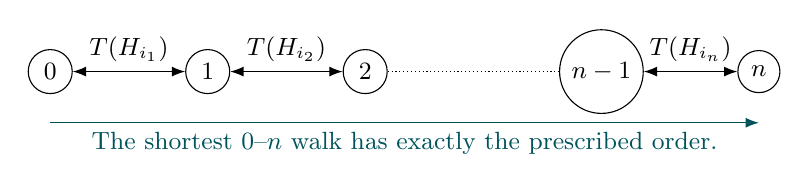
\begin{tikzpicture}[>=Latex,font=\small]
 \foreach \x/\lab in {0/0,2/1,4/2,7/{n-1},9/n}
   {\node[draw,circle,inner sep=3pt] (v\x) at (\x,0) {$\lab$};}
 \draw[<->] (v0)--node[above]{$T(H_{i_1})$}(v2);
 \draw[<->] (v2)--node[above]{$T(H_{i_2})$}(v4);
 \draw[densely dotted] (v4)--(v7);
 \draw[<->] (v7)--node[above]{$T(H_{i_n})$}(v9);
 \draw[->,linkteal] (0,-.65)--node[below]{The shortest $0$--$n$ walk has exactly the prescribed order.}(9,-.65);
\end{tikzpicture}
\caption{The reference path converts an ordered algebraic word into a coefficient of a physical information test. Backtracking walks enter only at higher orders.}
\label{fig:path}
\end{figure}

\begin{lemma}[Physical moment extraction]\label{lem:path}
The complete RLD profile determines every ordered moment
\[
 \tau\bigl(T(H_{i_1})\cdots T(H_{i_n})\bigr).
\]
Only the state \eqref{eq:path-state} and four families of traceless Hermitian tangents are needed for each word.
\end{lemma}

\begin{proof}
Write
\[
 Q_t=I-t\sum_{j=1}^nT(H_{i_j})\otimes A_j,
 \qquad C_t=(\tau\otimes\id_r)(Q_t^{-1}).
\]
For a rank-one reference projector $D$ define $K_D=I_a\otimes D-a\rho_t$. Its trace is zero. Expanding the quadratic form and using trace preservation yields
\begin{equation}\label{eq:path-readout}
 \rld_\E(\rho_t,K_D)+a^2
 =a^2r\Tr(D C_t).
\end{equation}
Indeed the raw tangent $I_a\otimes D$ gives the right side, and centering subtracts exactly $a^2$.

Take the projectors onto
\begin{equation}\label{eq:four-projectors}
 e_0,\quad e_n,\quad (e_0+e_n)/\sqrt2,\quad (e_0+\ii e_n)/\sqrt2.
\end{equation}
Their quadratic evaluations recover the complex $(0,n)$ entry of $C_t$. The Neumann expansion is norm convergent for $nt<1$. A walk from $0$ to $n$ has length at least $n$, and there is exactly one of length $n$. Consequently
\begin{equation}\label{eq:path-coefficient}
 [C_t]_{0n}
 =t^n\tau\bigl(T(H_{i_1})\cdots T(H_{i_n})\bigr)+O(t^{n+1}).
\end{equation}
Thus equality of physical profiles gives equality of the coefficient. No cyclic permutation of $\tau$ is used.
\end{proof}

For a word of length two, the reference has three vertices and the coefficient is $\tau(T(H_i)T(H_j))$. For length three it is $\tau(T(H_i)T(H_j)T(H_k))$, whose imaginary part can distinguish a channel from its transpose. The path is the self-adjoint, faithful-state version of the familiar matricial resolvent method for recovering noncommutative moments; see \cite{BPV}.

\subsection{From moments to the normal invariant}

\begin{lemma}\label{lem:moment-isomorphism}
Let two finite labelled self-adjoint families generate von Neumann algebras with faithful normal states. If all their ordered moments agree, there is a state-preserving normal $*$-isomorphism taking one labelled family to the other.
\end{lemma}

\begin{proof}
Evaluation of noncommutative $*$-polynomials gives the same seminorm $p\mapsto\tau(p^*p)^{1/2}$ in both systems. Faithfulness makes its null space precisely the polynomial relations. Hence the polynomial algebras are algebraically $*$-isomorphic.

This isomorphism also preserves the operator norm. For every polynomial value $p$,
\begin{equation}\label{eq:state-norm}
 \norm p=\lim_{k\to\infty}\tau((p^*p)^k)^{1/(2k)}.
\end{equation}
The upper bound is immediate. For the lower bound, every nonzero spectral projection of $p^*p$ near its spectral maximum has strictly positive state, by faithfulness; restricting to that projection proves the reverse inequality. This argument does not assume a trace. The algebraic isomorphism therefore extends isometrically to the generated $C^*$-algebras.

The matching states induce a unitary between the two GNS Hilbert spaces, intertwining left multiplication and the cyclic vectors. It extends the isomorphism to the generated von Neumann algebras. The GNS representation of a faithful normal state is faithful and normal, so this extension is a normal isomorphism of the original algebras.
\end{proof}

\begin{proof}[Proof of \cref{thm:classification}]
\Cref{lem:path,lem:moment-isomorphism} prove \textup{(i)}$\Rightarrow$\textup{(iii)}. A labelled normal state-preserving isomorphism preserves the bounded functional calculi in \eqref{eq:rld} and \eqref{eq:maxf}, also after tensoring with a finite matrix algebra. Thus \textup{(iii)} implies \textup{(i)} and \textup{(ii)}.

For the remaining implication choose $f_2(x)=(x-1)^2$. If $\rho$ is faithful and $K$ is a physical tangent, then $\rho+sK$ is faithful for sufficiently small real $s$, and the perspective formula gives the exact identity
\begin{equation}\label{eq:quadratic-identity}
 \maxdiv_{f_2}(\E_r(\rho+sK)\Vert\E_r(\rho))
 =s^2\rld_\E(\rho,K).
\end{equation}
Hence \textup{(ii)} implies \textup{(i)}. Tensoring the labelled isomorphism with itself proves the assertion for finite tensor powers. This concerns information profiles, not transmission capacities.
\end{proof}

\begin{example}[Why a reference is needed]\label{ex:transpose}
On $M_2$ let
\[
 \E(X)=\frac14X+\frac38\Tr(X)I_2,
 \qquad \F(X)=\E(X)^{\mathsf T}.
\]
Both are channels: their unnormalized Choi eigenvalues are respectively $7/8,3/8,3/8,3/8$ and $5/8,5/8,5/8,1/8$. Every unreferenced maximal $f$-divergence agrees because transpose preserves the perspective and the trace. Yet $\Omega=I_2$, $T_\E=\E$, and for the Pauli matrices
\[
 \tau(T_\E(\sigma_x)T_\E(\sigma_y)T_\E(\sigma_z))
 =\frac{\ii}{64},\qquad
 \tau(T_\F(\sigma_x)T_\F(\sigma_y)T_\F(\sigma_z))
 =-\frac{\ii}{64}.
\]
The length-three path, with a four-dimensional reference, separates them. Thus unreferenced equality cannot replace completeness.
\end{example}



% Included source: sections/04-finite
\section{The finite greatest representative}\label{sec:finite}

The normalized invariant separates two ingredients that a concrete output mixes together: the matrix blocks carrying the experiment, and the way those blocks are embedded and weighted in a Hilbert space. A greatest representative keeps each block once. Its postprocessing maps prepare every permitted embedding.

\subsection{Block preparation}

\begin{proof}[Proof of \cref{thm:finite}]
In the multiplicity-one representation, $h>0$ satisfies
\[
 \Tr(hZ)=a\tau(Z),\qquad \Tr(hT(X))=\Tr X.
\]
Consequently \eqref{eq:finite-canonical} is CPTP, its normalization is $T$, and its state is $\tau$. It belongs to the required class.

Let $\F$ be any realization \eqref{eq:all-realizations}, with representation $\pi$. Write $\pi_j$ for the representation of the $j$th block, extended by zero outside its central support. For $Y\in M_{n_j}$ define
\begin{equation}\label{eq:block-prep}
 \R_j(Y)=\Omega_\F^{1/2}
 \pi_j(h_j^{-1/2}Yh_j^{-1/2})\Omega_\F^{1/2}.
\end{equation}
This map is completely positive, and the prescribed state restriction gives
\[
 \Tr\R_j(Y)
 =\Tr(h_jh_j^{-1/2}Yh_j^{-1/2})=\Tr Y.
\]
Pinch the input onto its blocks and apply $\R_j$ to the $j$th block. The resulting CPTP map $\R$ satisfies $\R\Gamma=\F$. The target Hilbert space may be infinite; the formula still gives a trace-class output and a normal adjoint.

Finally, every realization contains a faithful representation of $\bigoplus_jM_{n_j}$. Each simple block must occur with positive multiplicity, so its output Hilbert space has dimension at least $\sum_jn_j$. The constructed representative attains this lower bound.
\end{proof}

The matrices $h_j$ need not be scalar. Replacing them by scalar block weights without traciality would change the profile and invalidate trace preservation in \eqref{eq:block-prep}.

\subsection{A concrete formula without choosing simple blocks}

Suppose $\E:M_a\to M_b$ has faithful $\Omega$. Let $\Pi:M_b\to\A$ be the ordinary trace-preserving conditional expectation onto $\A=C^*(T_\E(M_a))$, and put $Z=\Pi(\Omega)$. Finite-dimensional $\A$ has a unique such expectation: in a block decomposition it takes normalized partial traces over the multiplicity spaces. It is positive, faithful, and bimodular over $\A$.

\begin{proposition}[Concrete lift and transpose-channel reconstruction]\label{prop:concrete-lift}
The channel
\[
 \Gamma_\E(X)=Z^{1/2}T_\E(X)Z^{1/2}
\]
has the same profile as $\E$ and is greatest. It can be postprocessed to $\E$ by
\begin{equation}\label{eq:petz-lift}
 \R_\E(Y)=\Omega^{1/2}Z^{-1/2}\Pi(Y)Z^{-1/2}\Omega^{1/2}.
\end{equation}
If $\A=M_b$, then $\E$ itself is greatest.
\end{proposition}

\begin{proof}
Since $Z\in\A$ and $T_\E(X)\in\A$, normalization of $\Gamma_\E$ recovers $T_\E$. For $A\in\A$, trace preservation of $\Pi$ gives $\Tr(ZA)=\Tr(\Omega A)$, so the profile is unchanged. Complete positivity of \eqref{eq:petz-lift} is immediate. Its trace is
\[
 \Tr\R_\E(Y)
 =\Tr\bigl[\Pi(Y)Z^{-1/2}\Omega Z^{-1/2}\bigr]
 =\Tr\bigl[\Pi(Y)\Pi(Z^{-1/2}\Omega Z^{-1/2})\bigr]
 =\Tr Y,
\]
because bimodularity gives $\Pi(Z^{-1/2}\Omega Z^{-1/2})=I$. Substitution proves $\R_\E\Gamma_\E=\E$.

In a concrete block $M_{n_j}\otimes I_{m_j}$ the density is $Z_j=(h_j/m_j)\otimes I_{m_j}$. Thus $\Gamma_\E$ is the multiplicity-one greatest representative with a maximally mixed multiplicity factor attached. That factor can be discarded or prepared, so it remains greatest. If $\A=M_b$, then $\Pi=\id$ and $Z=\Omega$.
\end{proof}

Formula \eqref{eq:petz-lift} is the Petz transpose of the expectation with respect to $\Omega$, in the usual finite-dimensional form; see \cite[Theorem~3.18 and equations~(3.19)--(3.20)]{HiaiMosonyi}. It reconstructs $\E$ from a newly constructed channel $\Gamma_\E$. It does not assert that coarse-graining the actual outputs of $\E$ is sufficient.

\subsection{An elementary example of lost recoverability}

\begin{example}[Orthogonal records and nonorthogonal pure records]\label{ex:two-pure}
Let $\Gamma(X)=\diag(X_{00},X_{11})$. For $0<c<1$ set
\[
 \Omega_c=\begin{pmatrix}1&c\\c&1\end{pmatrix},\qquad
 \F_c(X)=\Omega_c^{1/2}\diag(X_{00},X_{11})\Omega_c^{1/2}.
\]
The diagonal entries of $\Omega_c$ are one, so $\F_c$ is trace preserving. Both channels have normalized map $T(X)=\diag(X_{00},X_{11})$ and the same state on the diagonal algebra. Hence their complete profiles agree.

For $c=3/5$ the formula is especially transparent:
\[
 \Omega_c^{1/2}=\frac1{\sqrt{10}}\begin{pmatrix}3&1\\1&3\end{pmatrix},\qquad
 \F_c(|0\rangle\langle0|)=\frac1{10}\begin{pmatrix}9&3\\3&1\end{pmatrix},\quad
 \F_c(|1\rangle\langle1|)=\frac1{10}\begin{pmatrix}1&3\\3&9\end{pmatrix}.
\]
The outputs are pure states with inner-product magnitude $3/5$. Their trace-norm distance is $8/5$, whereas the outputs of $\Gamma$ have distance $2$. No channel can convert the former pair to the latter. Thus $\Gamma\succeq\F_c$ but $\F_c\not\succeq\Gamma$, despite equality of every complete maximal-information profile. Both have the minimum effective output dimension, two.
\end{example}

The example also explains why a greatest representative is a mathematical reconstruction from a complete description. It is generally unavailable by deterministic processing of the given physical device. Profile equality is neither a recovery theorem nor a free channel-synthesis procedure.



% Included source: sections/05-exact
\section{Exact greatestness and atomicity}\label{sec:exact}

From this section through \cref{sec:examples}, the invariant state $\tau$ is a faithful normal \emph{trace}. The central device is a family of binary testing problems. Each one has a largest possible trace norm across the entire class, attained by a suitable pinched realization. A greatest member must attain all these bounds simultaneously.

\subsection{Pinching attains every testing bound separately}

\begin{lemma}[Testing envelope]\label{lem:bayes-envelope}
For every Hermitian input $X$ and every realization $\F$,
\begin{equation}\label{eq:bayes-upper}
 \norm{\F(X)}_1\le a\tau(\abs{T(X)}).
\end{equation}
For each fixed $X$, a realization in the same exact class attains equality.
\end{lemma}

\begin{proof}
Put $B=\pi_\F(T(X))$. Its positive and negative parts give
\[
 \F(X)=\Omega_\F^{1/2}B_+\Omega_\F^{1/2}
       -\Omega_\F^{1/2}B_-\Omega_\F^{1/2}.
\]
The triangle inequality proves \eqref{eq:bayes-upper}.

To attain it, start from one fixed realization $(\pi,\Omega)$, let $P=\one_{(0,\infty)}(\pi(T(X)))$, and define
\begin{equation}\label{eq:pinched-density}
 \Omega_P=P\Omega P+(I-P)\Omega(I-P).
\end{equation}
It is faithful: if its quadratic form vanishes at $\xi$, faithfulness of $\Omega$ forces both $P\xi=0$ and $(I-P)\xi=0$. Moreover, for every $Z\in\M$,
\[
 \Tr[\Omega_P\pi(Z)]
 =a\tau(P_0 ZP_0+(I-P_0)Z(I-P_0))=a\tau(Z),
\]
where $P_0$ is the corresponding projection of $\M$. This is precisely where traciality is used. Keeping $T$ fixed and replacing $\Omega$ by $\Omega_P$ therefore preserves the entire profile. The new density commutes with $P$, so the positive and negative output parts have orthogonal supports and equality holds.
\end{proof}

The bound $a\tau|T(X)|$ is an envelope over different physical realizations. There need not be one realization attaining it for every $X$.

\subsection{Simultaneous attainment forces a compact central density}

\begin{lemma}\label{lem:equality-commutes}
Let $\Omega$ be faithful trace class and $B=B^*$ bounded. If
\[
 \norm{\Omega^{1/2}(B-tI)\Omega^{1/2}}_1
 =\Tr(\Omega\abs{B-tI})
\]
for a dense set of thresholds $t$ with no spectral atom, then $\Omega$ commutes with $B$.
\end{lemma}

\begin{proof}
For a fixed threshold write $C=B-tI$. Equality in the trace-norm triangle inequality for the positive operators $A=\Omega^{1/2}C_+\Omega^{1/2}$ and $D=\Omega^{1/2}C_-\Omega^{1/2}$ implies that their supports are orthogonal. One way to see this is to use an optimal Helstrom projection $Q$: equality makes both errors $\Tr((I-Q)A)$ and $\Tr(QD)$ zero. Hence
\[
 C_+^{1/2}\Omega C_-^{1/2}=0.
\]
On the spectral subspaces $B\ge t+h$ and $B\le t-h$, the two square-root factors have bounded inverses. Thus the corresponding off-diagonal block of $\Omega$ is zero. Let $h\downarrow0$; absence of an atom at $t$ gives $[\Omega,\one_{(t,\infty)}(B)]=0$. Dense such cuts determine the spectral measure of $B$, and therefore $[\Omega,B]=0$.
\end{proof}

\begin{proof}[Necessity in \cref{thm:exact}]
Suppose $\G$ is greatest. For every Hermitian input $X$, the pinched target from \cref{lem:bayes-envelope} is a postprocessing of $\G$. Trace-norm contraction and \eqref{eq:bayes-upper} force $\G$ to attain the envelope at $X$.

Choose a finite Hermitian basis $H_i$ of the input and put $B_i=\pi_\G(T(H_i))$. Apply the preceding statement to $X=H_i-tI$. Each $B_i$ has at most countably many atoms under the faithful trace. The nonatom thresholds are dense, so \cref{lem:equality-commutes} gives $[\Omega_\G,B_i]=0$. Thus $\Omega_\G$ commutes with $\pi_\G(\M)$.

A faithful positive trace-class operator is compact. Its positive eigenspaces are finite dimensional and their orthogonal sum is the whole effective output space. They reduce $\pi_\G(\M)$, and the resulting finite-dimensional normal representations separate its points. For clarity, a normal representation onto a finite-dimensional algebra has a kernel which is a central ideal. Its complementary central support cuts out a finite-dimensional direct summand of $\M$. The central supports of the eigenspace representations have supremum one, because the representations separate points. Refining their countable union into minimal central summands shows that $\M$ is a countable product of finite matrix blocks. This proves \eqref{eq:atomic}.
\end{proof}

This compactness argument is the density-operator version of the established normal-projection obstruction. It excludes diffuse algebras even when they are injective.

\subsection{The countable block construction}

\begin{proof}[Sufficiency in \cref{thm:exact}]
Assume \eqref{eq:atomic}. Faithfulness and traciality give $\tau=\sum_jp_j\tr_{n_j}$ with all $p_j>0$. Formula \eqref{eq:atomic-channel} is CP and trace preserving because
\[
 \sum_j\frac{ap_j}{n_j}\Tr(T_j(X))=a\tau(T(X))=\Tr X.
\]
Its density is $\bigoplus_j(ap_j/n_j)I_{n_j}$ and its labelled invariant is the prescribed one.

For any target realization define on the $j$th input block
\[
 \R_j(Y)=\frac{n_j}{ap_j}\Omega_\F^{1/2}\pi_j(Y)\Omega_\F^{1/2}.
\]
Each is CPTP, by the trace restriction. Pinch onto the countably many blocks, then sum these maps. On positive trace-class inputs the sum converges in trace norm and preserves the trace. Linear extension gives a CPTP map with normal adjoint. Applied to \eqref{eq:atomic-channel} it yields $\F$. No global inverse of the block density is used; such an inverse could be unbounded.
\end{proof}



% Included source: sections/06-approximate
\section{Approximate greatestness and injectivity}\label{sec:approximate}

The exact proof required one compact density commuting with the entire invariant. Approximation asks for densities that commute with successively larger finite pieces. The subtle point is to obtain them without changing any of the prescribed information tests. Averaging over a finite unitary group does exactly this when $\tau$ is tracial.

\subsection{Finite quotients approximate every target uniformly}

Let $\M_k\subset\M$ be finite-dimensional unital subalgebras, increasing with weakly dense union. Write $\mathbb E_k:\M\to\M_k$ for the $\tau$-preserving conditional expectation. On $L^2(\M,\tau)$ it is the orthogonal projection, so
\begin{equation}\label{eq:L2-convergence}
 \norm{Z-\mathbb E_kZ}_{2,\tau}\longrightarrow0
 \quad(Z\in\M).
\end{equation}
If $\M_k=\bigoplus_jM_{n_{kj}}$ and $\tau|_{\M_k}=\sum_jp_{kj}\tr_{n_{kj}}$, set $h_{kj}=ap_{kj}/n_{kj}$ and
\begin{equation}\label{eq:external-lift}
 \Lambda_k(X)=\bigoplus_j h_{kj}[\mathbb E_kT(X)]_j.
\end{equation}
This is a finite-output channel. It is an auxiliary quotient and need not belong to the original profile class.

\begin{lemma}[Uniform external envelope]\label{lem:external-envelope}
For every realization $\F$ there is a CPTP map $\R_{k,\F}$ such that
\[
 \R_{k,\F}\Lambda_k(X)
 =\Omega_\F^{1/2}\pi_\F(\mathbb E_kT(X))\Omega_\F^{1/2}.
\]
Uniformly over all target realizations,
\begin{equation}\label{eq:uniform-error}
 \norm{\F-\R_{k,\F}\Lambda_k}_\diamond
 \le\varepsilon_k:={a}\sum_{i,j=1}^a
 \norm{T(E_{ij})-\mathbb E_kT(E_{ij})}_{2,\tau}
 \longrightarrow0.
\end{equation}
\end{lemma}

\begin{proof}
Use the block preparation map \eqref{eq:block-prep} for $\M_k$, where $h_j=h_{kj}I$. It is trace preserving on each block and gives the displayed formula.

For $B\in\M$, the Schatten Cauchy--Schwarz inequality and the trace restriction give
\begin{equation}\label{eq:sandwich-L2}
 \norm{\Omega_\F^{1/2}\pi_\F(B)\Omega_\F^{1/2}}_1
 \le a\norm B_{2,\tau}.
\end{equation}
For example, factor the product into the Hilbert--Schmidt operators $\Omega_\F^{1/2}\pi_\F(B)$ and $\Omega_\F^{1/2}$. For an arbitrary referenced input $Z=\sum_{ij}E_{ij}\otimes Z_{ij}$, each $\norm{Z_{ij}}_1\le\norm Z_1$. Apply \eqref{eq:sandwich-L2} to each matrix unit and sum. This proves the diamond bound independently of the target output space and of the reference dimension. Equation \eqref{eq:L2-convergence} proves its limit.
\end{proof}

\subsection{Keeping the sources in the exact class}

\begin{proof}[\textup{(iii)}$\Rightarrow$\textup{(i)} in \cref{thm:approximate}]
The exact structural import is Connes' theorem \cite[Chapter~V, \S7, Theorem~6]{Connes}: a von Neumann algebra acting on a separable Hilbert space is injective if and only if it is approximately finite dimensional. It applies here because $\M$ acts on the given separable effective output space. In the finite tracial case it yields the sequence of finite-dimensional subalgebras used above; adjoining the ambient identity if necessary makes them unital. Weak density implies $L^2(\tau)$ density, and the trace supplies the expectations $\mathbb E_k$. No effective form of this theorem is used.

Fix one realization $(\pi,\Omega)$ and identify $\M$ with its image. Haar-average the trace-class density over the compact finite-dimensional unitary group:
\begin{equation}\label{eq:Haar-density}
 \Omega^{(k)}=\int_{\mathcal U(\M_k)}u\Omega u^*\,\dd u.
\end{equation}
This is a trace-norm Bochner integral. It is faithful: for nonzero $\xi$, the integrand's quadratic form is everywhere strictly positive. It commutes with $\M_k$. More importantly, for every $Z\in\M$,
\[
 \Tr(\Omega^{(k)}Z)
 =a\int\tau(u^*Zu)\,\dd u=a\tau(Z).
\]
Thus
\begin{equation}\label{eq:inside-source}
 \G_k(X)=(\Omega^{(k)})^{1/2}T(X)(\Omega^{(k)})^{1/2}
\end{equation}
belongs to the \emph{exact} original profile class for every $k$.

Decompose the representation of $\M_k$ as
\[
 \HH=\bigoplus_j(\mathbb C^{n_{kj}}\otimes\mathcal K_{kj}),\qquad
 \Omega^{(k)}=\bigoplus_j(I_{n_{kj}}\otimes\omega_{kj}),
 \quad\Tr\omega_{kj}=h_{kj}.
\]
Block pinching followed by the usual partial trace defines a normal CPTP map $S_k$ to $\bigoplus_jM_{n_{kj}}$. For $Y\in\M_k$, its output satisfies
\begin{align*}
 \Tr[S_k\G_k(X)Y]
 &=\Tr[\Omega^{(k)}T(X)Y]\\
 &=a\tau(T(X)Y)=a\tau(\mathbb E_kT(X)Y).
\end{align*}
The first equality uses commutation with $\M_k$, and the last is the defining property of the expectation. Hence $S_k\G_k=\Lambda_k$. Combining this identity with \cref{lem:external-envelope} gives
\[
 \sup_{\F\in\C}\defic(\G_k,\F)\le\varepsilon_k\longrightarrow0.
\]
This proves \textup{(i)}. Choosing errors tending to zero proves \textup{(i)}$\Rightarrow$\textup{(ii)}.
\end{proof}

\subsection{Testing deficits force near-centrality}

We next prove the converse. Its targets are fixed in advance; no uniform convergence assumption will enter.

At a threshold $t$, the positive and negative parts of $B-tI$ define a binary testing problem. A pinched realization makes their records orthogonal, so its testing norm reaches the class-wide bound. A source that nearly simulates this target must nearly reach the same bound. Its optimal test then makes few errors on the two parts. The estimate below turns those errors into a small overlap, and then into a small off-diagonal block of $\Omega$ across the spectral cut. Repeating the argument at dense thresholds forces the density to almost commute with every generator. This is the operational input to the central-state argument; the latter is established amenability theory.

\begin{lemma}[A quantitative spectral-cut estimate]\label{lem:cut-estimate}
Let $B=B^*\in\M$, let $(\pi,\Omega)$ be a realization of $a\tau$, and fix $t\in\mathbb R$. Define
\[
 s=a\tau|B-tI|,\qquad
 \Delta=s-\norm{\Omega^{1/2}\pi(B-tI)\Omega^{1/2}}_1.
\]
For $P_t=\one_{(t,\infty)}(B)$ and every $h>0$,
\begin{equation}\label{eq:cut-bound}
 \norm{[\Omega,\pi(P_t)]}_1
 \le\frac{2\sqrt{s\Delta/2}}h
       +4a\sqrt{\tau(\one_{[t-h,t+h]}(B))}.
\end{equation}
\end{lemma}

\begin{proof}
Put $C=\pi(B)-tI$, $A=\Omega^{1/2}C_+\Omega^{1/2}$, and $D=\Omega^{1/2}C_-\Omega^{1/2}$. An optimal Helstrom projection $Q$ for $A-D$ satisfies
\[
 e_A:=\Tr((I-Q)A),\quad e_D:=\Tr(QD),\quad e_A+e_D=\Delta/2.
\]
With $x=\Omega^{1/2}C_+^{1/2}$ and $y=\Omega^{1/2}C_-^{1/2}$, split $x^*y$ at $Q$. Schatten Cauchy--Schwarz gives
\begin{align}
 \norm{C_+^{1/2}\Omega C_-^{1/2}}_1
 &\le\sqrt{\Tr(A)e_D}+\sqrt{\Tr(D)e_A}
 \le\sqrt{s\Delta/2}.\label{eq:Helstrom-overlap}
\end{align}
On the cuts $B>t+h$ and $B<t-h$, inverse square roots have norm at most $h^{-1/2}$. The far off-diagonal block of $\Omega$ is therefore bounded by the right side of \eqref{eq:Helstrom-overlap} divided by $h$. Each of the two remaining near-cut blocks is bounded by
\[
 \norm{\pi(N)\Omega^{1/2}}_2\norm{\Omega^{1/2}}_2
 \le a\sqrt{\tau(N)},\qquad N=\one_{[t-h,t+h]}(B).
\]
The trace norm of the commutator is twice the norm of its off-diagonal block. Summing the three bounds proves \eqref{eq:cut-bound}, including possible mass at $t$.
\end{proof}

\begin{proof}[\textup{(ii)}$\Rightarrow$\textup{(iii)} in \cref{thm:approximate}]
Choose a Hermitian input basis $H_i$ and write $B_i=T(H_i)$. For each $i$ choose a countable dense set of thresholds having no atom in the $\tau$-spectral measure of $B_i$. Using one fixed base density, pinch it at each $P_{it}=\one_{(t,\infty)}(B_i)$ as in \eqref{eq:pinched-density}. Denote these fixed class targets by $\F_{it}$. They attain the testing envelope at $X_{it}=H_i-tI$.

Write $\G_k(X)=\Omega_k^{1/2}\pi_k(T(X))\Omega_k^{1/2}$. Since $\defic(\G_k,\F_{it})\to0$, contractivity of a nearly optimal decoder gives
\[
 0\le\Delta_{kit}:=a\tau|B_i-tI|-\norm{\G_k(H_i-tI)}_1
 \le\norm{H_i-tI}_1\bigl(\defic(\G_k,\F_{it})+1/k\bigr)
 \longrightarrow0.
\]
Apply \cref{lem:cut-estimate}. First take $k\to\infty$ at fixed $h$, then $h\downarrow0$. Nonatomicity at $t$ yields
\[
 \norm{[\Omega_k,\pi_k(P_{it})]}_1\longrightarrow0.
\]
Step-function approximation along dense thresholds gives the same limit for each generator $B_i$. Commutator identities then give it for all noncommutative polynomials and the generated $C^*$-algebra.

The extension to the full von Neumann algebra is uniform in $k$. Indeed, \eqref{eq:sandwich-L2} and a Hilbert--Schmidt factorization give
\begin{equation}\label{eq:comm-L2}
 \norm{[\Omega_k,\pi_k(Z)]}_1\le2a\norm Z_{2,\tau}.
\end{equation}
Kaplansky density supplies bounded $C^*$-algebra approximants to any $Z\in\M$ in $L^2(\tau)$. Applying \eqref{eq:comm-L2} to their differences proves centrality for every $Z$.

On $\mathcal K=\bigoplus_k\HH_k$, let $\pi=\bigoplus_k\pi_k$. It is faithful and normal. The states supported in the $k$th summand with density $\Omega_k/a$ restrict exactly to $\tau$ on $\pi(\M)$ and become central there. A weak-$*$ cluster subnet in the state space of $\B(\mathcal K)$ gives a state $\varphi$ such that
\begin{equation}\label{eq:hypertrace}
 \varphi(\pi(Z))=\tau(Z),\qquad
 \varphi(A\pi(Z))=\varphi(\pi(Z)A).
\end{equation}
No sequential compactness or normality of $\varphi$ is asserted.

We include the standard projection argument to specify exactly what is obtained. For $A\ge0$, the functional $Z\mapsto\varphi(A\pi(Z))$ is positive on $\M$: for $Z\ge0$, centrality rewrites it as $\varphi(\pi(Z)^{1/2}A\pi(Z)^{1/2})$. It is bounded above by $\norm A\tau(Z)$. Domination by a normal trace makes it normal, with a unique bounded positive Radon--Nikodym density $P(A)\in\M$ satisfying
\[
 \tau(P(A)Z)=\varphi(A\pi(Z)).
\]
Extend linearly. Uniqueness shows that $P$ is unital, fixes $\M$, and is bimodular. If $[A_{ij}]\ge0$ and $m_i\in\M$, then
\[
 \tau\!\left(\sum_{ij}m_i^*P(A_{ij})m_j\right)
 =\varphi\!\left(\sum_{ij}\pi(m_i)^*A_{ij}\pi(m_j)\right)\ge0.
\]
The vectors $m_i$ are dense in $L^2(\M,\tau)$, so $P$ is completely positive. Thus $\pi\circ P$ is a UCP projection from $\B(\mathcal K)$ onto $\pi(\M)$. This is injectivity. The projection need not be normal, which is consistent with the diffuse cases excluded by \cref{thm:exact}.
\end{proof}

\begin{proof}[Proof of \cref{cor:finite-obstruction}]
Enumerate the countable fixed cut targets used in the converse. If no finite subfamily had a positive simultaneous obstruction, for each $k$ there would be a class source approximating the first $k$ targets within $1/k$. The same near-centrality proof would yield injectivity. Its contrapositive gives the assertion. This argument provides neither an effective list nor an effective gap; \cref{app:free-group} gives both for one explicit invariant.
\end{proof}



% Included source: sections/07-examples
\section{Diffuse and noninjective examples}\label{sec:examples}

The realization criteria are not restricted to abstract operator algebras. A binary input already exhibits the difference between exact and approximate greatestness. A three-dimensional input realizes the free-group obstruction.

\subsection{A binary diffuse class}

Let $\nu$ be normalized Lebesgue measure on $[1/4,3/4]$, let $\HH=L^2(\nu)$, and write $A$ for multiplication by the coordinate. The vectors
\[
 e_n(x)=\exp(4\pi\ii n(x-1/4)),\qquad n\in\mathbb Z,
\]
form an orthonormal basis. Set
\[
 \Omega=\sum_{n\in\mathbb Z}\frac23\,2^{-|n|}|e_n\rangle\langle e_n|,
 \quad\rho_0=\Omega^{1/2}A\Omega^{1/2},\quad
 \rho_1=\Omega^{1/2}(I-A)\Omega^{1/2}.
\]
The density $\Omega$ is faithful, has trace $2$, and satisfies
\[
 \frac12\Tr(\Omega f(A))=\int f(x)\,\dd\nu(x).
\]
Both $\rho_i$ have trace one, and $\Omega/4\le\rho_i\le3\Omega/4$. Thus
\begin{equation}\label{eq:diffuse-binary}
 \E(X)=X_{00}\rho_0+X_{11}\rho_1
\end{equation}
is an ordinary channel with faithful output states. Its invariant is
\[
 T(X)=X_{00}A+X_{11}(I-A),\qquad
 \M=L^\infty(\nu),\qquad\tau(f)=\int f\,\dd\nu.
\]
It has no greatest density-operator realization by \cref{thm:exact}. Dyadic step functions generate $L^\infty(\nu)$ weakly, so the invariant is hyperfinite and \cref{thm:approximate} applies.

The approximation can be seen directly. Partition the interval into bins of width at most $h$. For a bin $I_j$, put $\mu_j=\nu(I_j)$ and $\lambda_j=\mu_j^{-1}\int_{I_j}x\,\dd\nu(x)$. The finite classical channel with columns
\[
 \bigl(2\mu_j\lambda_j\bigr)_j,
 \qquad \bigl(2\mu_j(1-\lambda_j)\bigr)_j
\]
can simulate any realization of \eqref{eq:diffuse-binary} within diamond error $2h$: prepare from bin $j$ the density
\[
 \frac{\Omega_\F^{1/2}\pi_\F(\one_{I_j}(A))\Omega_\F^{1/2}}{2\mu_j}.
\]
The reconstructed coordinate differs from $A$ in norm by at most $h$, which gives the bound by trace-norm sandwiching. This finite channel is an external envelope, not an exact member of the diffuse class. The Haar construction supplies sources \emph{inside} that class which process to it.

More generally, a binary measure-and-prepare channel has $T(|0\rangle\langle0|)=A$, $T(|1\rangle\langle1|)=I-A$. Its invariant is determined by
\[
 \mu(B)=\frac12\Tr(\Omega\one_B(A)),\qquad \int x\,\dd\mu(x)=\frac12.
\]
Its greatest trace-class realization exists exactly when $\mu$ is purely atomic. In the atomic case the greatest output distributions are $2\mu_j\lambda_j$ and $2\mu_j(1-\lambda_j)$. This is the familiar spectral reverse experiment. For a diffuse $\mu$ a generalized $L^\infty$-valued reverse experiment still exists; the obstruction concerns representing its classical outcomes by ordinary density matrices, not the existence of the generalized experiment \cite{Matsumoto,Hiai,Holevo}.

\subsection{A three-input free-group class}

Let $\mathbb F_2=\langle u,v\rangle$, and let $U,V$ be its left regular unitaries on $\ell^2(\mathbb F_2)$. The group von Neumann algebra $L(\mathbb F_2)$ has its canonical faithful normal trace $\tau$.

\begin{proposition}\label{prop:free-group}
There is a channel $\E:M_3\to\Sone(\ell^2(\mathbb F_2))$ with invariant $(L(\mathbb F_2),T,\tau)$, where
\begin{equation}\label{eq:free-Choi}
 J_T=
 \begin{pmatrix}
 I/3&U/12&V/12\\
 U^*/12&I/3&0\\
 V^*/12&0&I/3
 \end{pmatrix},\qquad
 \Omega_{g,g}=\frac{3}{5\cdot4^{|g|}}.
\end{equation}
Its profile class has no common pointwise approximating greatest sequence. In fact there are sixty explicit fixed targets in the class such that, for every class member $\G$,
\begin{equation}\label{eq:60-gap}
 \max_{1\le j\le60}\defic(\G,\F_j)
 >\frac{3}{13\cdot2^{34}}.
\end{equation}
\end{proposition}

\begin{proof}
The row operator $[U,V]$ has norm $\sqrt2$, so
\[
 J_T\ge\frac{4-\sqrt2}{12}I.
\]
Thus $T$ is CP and $T(I_3)=I$. The number of reduced words of length $n\ge1$ is $4\cdot3^{n-1}$, whence $\sum_g4^{-|g|}=5$ and $\Tr\Omega=3$. Every diagonal coefficient of an element of $L(\mathbb F_2)$ is its canonical trace. Consequently $\Tr(\Omega Z)=3\tau(Z)$ and $3\tau(T(E_{ij}))=\delta_{ij}$. Therefore $\E(X)=\Omega^{1/2}T(X)\Omega^{1/2}$ is CPTP. The off-diagonal labels recover $U,V$, so the generated algebra is exactly $L(\mathbb F_2)$.

For completeness, noninjectivity follows from the usual invariant-mean obstruction. A UCP projection from $\B(\ell^2(\mathbb F_2))$ onto $L(\mathbb F_2)$ would, after restriction to diagonal multiplication operators and composition with $\tau$, give a left-invariant mean on $\ell^\infty(\mathbb F_2)$. Bimodularity follows from the multiplicative domain of a UCP map fixing the algebra. Let $W_s$ be the nonempty reduced words beginning with $s$. The relation
\[
 u(\mathbb F_2\setminus W_{u^{-1}})=W_u
\]
would give $m(W_u)+m(W_{u^{-1}})=1$, and the analogous relation for $v$ gives another sum of one. The four sets are disjoint and cover the group except the identity, whose invariant mean is zero. Their total mean cannot be both one and two. Thus the algebra is noninjective, and \cref{thm:approximate} gives the qualitative conclusion. The quantitative form \eqref{eq:60-gap} is proved in \cref{app:free-group}.
\end{proof}

This channel has an effective infinite description. In the word basis,
\[
 [\E(E_{ii})]_{g,g}=\frac1{5\cdot4^{|g|}},\qquad
 [\E(E_{01})]_{g,h}=
 \begin{cases}
 (20\cdot2^{|g|+|h|})^{-1},&g=uh,\\0,&g\ne uh,
 \end{cases}
\]
with the analogous formula for $E_{02}$. The density tail is
\[
 \Tr(\one_{\{|g|>L\}}\Omega)=\frac{12}{5}(3/4)^L.
\]
These are computable rational matrix entries with a controlled tail, not a finite rational Choi matrix. The positive floor in \eqref{eq:free-Choi} is a floor for the \emph{bounded normalized} Choi operator. The physical Choi operator has only a relative lower bound proportional to $I_3\otimes\Omega$; an absolute positive floor is impossible in infinite dimension.



% Included source: sections/08-stability
\section{Exact identification and unstable optimization}\label{sec:stability}

The classification theorem is exact. It has an effective finite-dimensional version, but exact computability does not imply stability under finite experimental precision. We first state what can be identified, then give a full-support example showing why a conditioning assumption is unavoidable.

\subsection{Finite descriptions and finite tests}

\begin{theorem}[Exact finite-channel equality and physical witnesses]\label{thm:algorithm}
Given two finite channels by rational complex Choi matrices, equality of their complete profiles can be decided in polynomial time in the explicit matrix dimensions and bit length. If they differ, a polynomial-time algorithm produces a finite reference, rational faithful input densities, and a rational physical tangent separating their RLD and maximal quadratic profiles. If the effective output ranks are $b_\E,b_\F$, the reference dimension is at most $b_\E^2+b_\F^2$. The witness has polynomial bit length, but its information gap need not be bounded below by an inverse polynomial.
\end{theorem}

The algorithm uses finite-dimensional word-space closure, the same principle used in equivalence algorithms for linear and quantum sequential machines \cite[Theorem~2]{LiQiu}. The additional step converts a separating word into faithful physical tests. We give the complete algorithm and gap bound in \cref{app:witnesses}. This is an exact description model, not an assertion about the number of black-box channel uses.

There is also a finite universal probe family at fixed dimensions. Put $m=a^2(b^2-1)$ and fix a rational $\lambda>0$. On the compact set of CPTP maps $M_a\to M_b$ with $\E(I)\ge\lambda I$, there exist $2m+1$ rational faithful RLD probes, with reference dimension $2b^2$, which separate all exact profile classes. They can be found by enumeration and real quantifier elimination. This is an application of the analytic identification principle behind Sontag's $2m+1$ theorem \cite[Theorem~2]{Sontag}; the count is not a new identification principle. Offline search and measurement precision have no polynomial bound here.

For noisy data one can impose a quantitative algebra-generation condition. Form the matrix $V_\E$ whose columns are the vectorized normalized words of length at most $b^2-1$, including the identity. If
\begin{equation}\label{eq:conditioning}
 \E(I)\ge\lambda I,\qquad V_\E V_\E^*\ge\kappa I_{b^2},
 \quad\lambda,\kappa>0,
\end{equation}
then finitely many RLD measurements control the channel up to an output unitary by a H\"older bound. The exponent and constant are effective semialgebraic quantities. \Cref{app:probes} states and proves these assertions precisely using the established \L ojasiewicz inequality \cite[Theorem~2.2]{BasuMN}. The constants may deteriorate as $\kappa\downarrow0$.

\subsection{A full-support discontinuity}

For a finite-output class let
\[
 Q_*(\E)=\sup\{Q(\F):\F\sim\E,\ \F\text{ has finite output}\},
\]
where $Q$ is unassisted quantum capacity. By \cref{thm:finite}, this supremum equals $Q(\Gamma)$ for a greatest representative. Also define the optimized singlet fraction
\[
 f_*(\E)=\sup_{\F\sim\E,\ \mathsf D}
 \langle\phi_2|(\id_2\otimes\mathsf D\F)(|\phi_2\rangle\langle\phi_2|)|\phi_2\rangle,
\]
for qubit input, with $\mathsf D$ a CPTP decoder to a qubit and $\phi_2=(|00\rangle+|11\rangle)/\sqrt2$. Allowing all separable outputs in this second supremum gives the same value, because the finite greatest representative simulates them.

\begin{theorem}[A fixed full-support family]\label{thm:instability}
There is an explicit affine family $\E_t:M_2\to M_4$, $0\le t\le2^{-16}$, rational for rational $t$, with the following properties. Put
\[
 \Omega=\frac1{14}\diag(25,1,1,1),\qquad
 \Delta(X)=\frac78X+\frac1{16}\Tr(X)I_2.
\]
For every allowed $t$,
\[
 \E_t(I)=\Omega,\qquad J_{\E_t}\ge I_8/448,\qquad
 \norm{\E_t-\E_0}_\diamond\le2t,
\]
and $\E_t$ is antidegradable, hence $Q(\E_t)=0$. At $t=0$, $\E_0\sim\Delta$ and the greatest representative has minimum dimension two. For every $t>0$ in the interval, $\E_t$ itself is greatest and its minimum output dimension is four. Moreover,
\begin{align}
 f_*(\E_0)&=29/32,& f_*(\E_t)&\le3/4\quad(t>0),\label{eq:f-jump}\\
 Q_*(\E_0)&>25/64,& Q_*(\E_t)&=0\quad(t>0),\label{eq:Q-jump}\\
 \defic(\E_t,\Delta)&\ge5/16,&
 \defic(\Delta,\E_t)&\le2t.\label{eq:asymmetric-gap}
\end{align}
The complete formulas and positivity certificates are given in \cref{app:instability}.
\end{theorem}

\begin{proof}[Operational part of the proof]
\Cref{app:instability} constructs the affine family, proves a full-space symmetric extension of its Choi matrices, and verifies that its normalized algebra is a copy of $M_2$ at zero and all of $M_4$ at every positive $t<1$. The finite greatest-representative theorem gives the stated canonical outputs.

A channel is antidegradable if and only if its Choi state has a symmetric extension to two whole output systems \cite[Lemma~5]{MyhrLutkenhaus}. To see the needed implication, regard the extension as a broadcasting channel with both marginals $\E_t$. A Stinespring dilation of it contains a complementary output of one marginal from which the other marginal is obtained by partial trace. Uniqueness of Stinespring dilation transfers this map to a complement of $\E_t$. Thus $\E_t$ is antidegradable. For a purified input, data processing bounds the coherent information to its output by the coherent information to its complement; purity makes the latter the negative of the former. It is therefore nonpositive. Tensor powers remain antidegradable, so the regularized coherent-information formula \cite{Devetak} gives zero unassisted quantum capacity.

Any decoded qubit Choi state of an antidegradable channel still has a two-output symmetric extension. Let $P_1$ and $P_2$ be the maximally entangled projectors on the input qubit and respectively the first and second output qubits, tensored with identity on the remaining output. The identity $P_1P_2P_1=P_1/4$ implies $\norm{P_1+P_2}=3/2$. Equal marginals therefore have singlet fraction at most $3/4$. This proves the positive-$t$ bound in \eqref{eq:f-jump}.

The identity decoder for $\Delta$ gives $29/32$. It is optimal: for any qubit decoder the identity-channel component has singlet fraction at most one, and the replacer component has singlet fraction exactly $1/4$. Their convex combination is at most $7/8+(1/8)/4=29/32$. Since $\Delta$ is greatest at zero, this proves equality in \eqref{eq:f-jump}. The gap $5/32$ in one effect evaluation is at most half the trace distance between normalized Choi states, hence at most half the diamond distance. This gives the first part of \eqref{eq:asymmetric-gap}. The other follows by processing $\Delta$ to $\E_0$ and using $\norm{\E_t-\E_0}_\diamond\le2t$.

Finally, the coherent information of $\Delta$ at the maximally mixed input is
\[
 1-H(29/32,1/32,1/32,1/32)>25/64.
\]
Indeed $-(29/32)\log_2(29/32)\le(3/32)\log_2\ee<9/64$, and the three remaining entropy terms sum to $15/32$. Coherent information is an achievable quantum rate \cite[Theorem~5 and Proposition~7]{Devetak}. The capacity claims now follow from greatestness and antidegradability.
\end{proof}

The discontinuous quantity is the capacity optimized over an \emph{exact information class}. The ordinary capacity of the physical channels is zero throughout. Thus this example is consistent with finite-dimensional continuity of quantum capacity \cite[Corollary~14]{LeungSmith}. It also shows that a fixed Choi floor and a fixed faithful output density do not control exact canonicalization: the generated algebra can change discontinuously.

\subsection{The acquisition cost of an exact distinction}

\begin{proposition}[Black-box distinction along the fixed family]\label{prop:acquisition}
For $t=2^{-m}$, $m\ge16$, any adaptive procedure distinguishing $\E_0$ from $\E_t$ with success probability at least $2/3$ under equal priors requires
\[
 N\ge\frac{\log(13/9)}{\log(1+(512t)^2)}>2^{2m-20}
\]
channel uses. A nonadaptive experiment achieves this with $O(t^{-2})$ uses.
\end{proposition}

\begin{proof}
Write $\E_t=\E_0+tG$, where $G=\R-\E_0$ and $\R$ is the endpoint channel in \cref{app:instability}. Put $s=1/512$ and $\E_\pm=\E_0\pm sG$. They are CPTP: $\norm{J_G}\le2$, while $J_{\E_0}\ge I/224$, so $J_{\E_-}\ge I/1792$; $\E_+$ is a convex combination of channels. The map $\E_t$ is the mixture of $\E_\pm$ with selector probabilities $(1\pm512t)/2$.

Give an adaptive experiment the selector coin for every use. Conditional on these independent coins, its complete output is obtained by a fixed quantum processing. Its distinguishability is consequently no greater than that of $N$ independent fair coins versus coins of bias $512t$. Their product chi-square divergence is $(1+(512t)^2)^N-1$, and total variation is at most half its square root. Success $2/3$ requires variation at least $1/3$, proving the logarithmic bound. Since $\log(1+x)\le x$ and $\log(13/9)>1/4$, the displayed strict power-of-two bound follows.

For the upper bound, input $|0\rangle$ and measure the first output basis projector. Its success probability is $25/28-75t/6272$, by the formulas in \cref{app:instability}. A standard Hoeffding test separates the two probabilities with $O(t^{-2})$ samples.
\end{proof}

The reduction from adaptive channel discrimination to program-state discrimination is established machinery; see \cite[Theorem~3]{JiEtAl} and the classical-simulation method in \cite{Demkowicz}. Here it quantifies the experimental cost of resolving the exact algebra change in one fixed, uniformly full-support family. An input parameter with $O(m)$ bits can therefore encode a profile change whose direct acquisition requires exponentially many uses.



% Included source: sections/09-discussion
\section{Consequences, limitations, and open questions}\label{sec:discussion}

\subsection{A routine consequence for finite capacity spectra}

The greatest representative determines the upper capacity allowed by a finite-dimensional profile. The lower end can approach zero within the same exact class. This is a consequence of an invertible Bell filter and continuity, rather than a separate capacity formula.

\begin{proposition}\label{prop:capacity-spectrum}
Let a profile class have a finite-dimensional invariant, and let $\Gamma$ be its greatest representative. Among finite-output members its quantum-capacity spectrum is $\{0\}$ if $Q(\Gamma)=0$. Otherwise it is either $(0,Q(\Gamma)]$ or $[0,Q(\Gamma)]$. In particular every strictly positive value below $Q(\Gamma)$ occurs. The statement allows arbitrary real channel coefficients; a rational parameter restriction need only give a dense set of values.
\end{proposition}

\begin{proof}
Let the effective output dimension of $\Gamma$ be $b$. On $\mathbb C^b\otimes\mathbb C^b$ write $P_b=|\phi_b\rangle\langle\phi_b|$ for the normalized maximally entangled projector, and set
\[
 S_u=uI+P_b,\qquad
 \kappa_u=bu^2+(2u+1)/b,\qquad
 \F_u(X)=\kappa_u^{-1}S_u(\Gamma(X)\otimes I_b)S_u.
\]
Since $\Tr_2S_u^2=\kappa_u I_b$, this is a channel. For $u>0$, put
\[
 A_u=\kappa_u^{-1/2}S_u(\Omega_\Gamma^{1/2}\otimes I_b).
\]
Its polar decomposition is $A_u=\Omega_{\F_u}^{1/2}U_u$ with $U_u$ unitary. Normalizing $\F_u$ therefore gives $U_u(T_\Gamma(\cdot)\otimes I_b)U_u^*$. The partial-trace identity shows that its state on this labelled algebra is precisely $\tau_\Gamma$. Thus $\F_u\sim\Gamma$ for every $u>0$.

At $u=0$ the same formula is the pure replacer $X\mapsto\Tr(X)P_b$. Hence $\F_u$ approaches that replacer in diamond norm, and $Q(\F_u)\to0$ by fixed-output capacity continuity \cite[Corollary~14]{LeungSmith}. No claim of profile equality is made at $u=0$.

If $\E,\F$ are in the class, their flagged interpolation $(1-t)\E\oplus t\F$ is in the class for $0<t<1$: its normalized algebra is the diagonal graph of the common labelled invariant, and its state is $(1-t)\tau+t\tau=\tau$. The endpoints belong as well, with their effective supports. The capacity along this finite-output path is continuous. Interpolating between $\Gamma$ and members of arbitrarily small capacity yields every strictly intermediate value. Greatestness bounds all capacities above by $Q(\Gamma)$. Whether zero itself occurs is the only remaining alternative.
\end{proof}

\subsection{What the realization theorems do and do not identify}

The physical reference tests recover a labelled normal algebra and state. In finite dimensions this is enough to construct a greatest representative from an exact description. It is not enough to recover that representative from an arbitrary member by deterministic processing; \cref{ex:two-pure} rules this out. Optimizing over the profile class is a change of realization, not an available operation on the original device.

The infinite-dimensional approximation theorem has equally specific quantifiers. One source must approximate every fixed target, and its exact complete profile is prescribed. Choosing a different source for each target would make the pointwise statement vacuous: the target itself could be chosen. The positive theorem constructs a sequence with a uniform target-independent error bound, while its converse requires only a common pointwise sequence. It supplies no finite-dimensional exact representative of a diffuse invariant and no algorithm for recognizing injectivity from an infinite presentation.

The strongest comparisons in the literature explain substantial parts of this picture. Generalized reverse tests permit diffuse classical outputs. Normal projection and instrument-extension theorems already distinguish atomic exact realizations from injective approximate ones. The same-profile requirement and the finite-input diamond estimates specify how those structures govern the present channel class. No claim that the underlying atomic/injective distinction, amenability characterization, resolvent principle, word-closure algorithm, generic probe count, or semialgebraic error-bound mechanism is new is intended.

\subsection{Decisive remaining questions}

The first structural question is the infinite-output \emph{nontracial} case. Finite block preparation works with arbitrary faithful block densities, but the two infinite arguments use traciality in different ways: spectral pinching must preserve the state on every label, and Haar averaging must preserve its restriction to the whole invariant. A replacement would have to respect the modular structure of a nontracial state. Ordinary sufficiency results based on cocycles suggest relevant machinery, but do not establish the greatest-member criterion for this larger profile class.

The second question is effective approximation. A supplied hyperfinite filtration gives the explicit bound \eqref{eq:uniform-error}. Injectivity alone supplies neither a computable filtration nor a modulus. An effective presentation with a verified $L^2$ approximation procedure would turn the existence theorem into a channel compiler; a bare matrix-entry description is insufficient. The binary bins in \cref{sec:examples} illustrate the extra information that makes a constructive rate possible.

The third question concerns robust optimization. \Cref{thm:instability} excludes a uniform continuity theorem based only on positive Choi and output-density floors. The conditioned estimate in \cref{app:probes} applies on a full-algebra stratum. A useful extension would identify a physically verifiable distance from changes of algebra type and then quantify the cost of certifying that condition. Exact algebraic equality and low-precision experimental identification must remain distinct.

Finally, the capacity spectrum leaves a precise endpoint problem: when $Q(\Gamma)>0$, must the class contain an exactly zero-capacity finite realization? The Bell filter proves arbitrarily small capacity, and \cref{thm:instability} supplies a class where zero is attained. Neither argument settles the endpoint for every class. Determining it would require a property beyond continuity.


\section*{Acknowledgements and AI use}
The mathematical ideas, constructions, proofs, and manuscript were developed by GPT-6 Astra, with additional AI assistance for review. Human input was minimal and consisted primarily of setting the research objectives and providing occasional feedback.
\appendix

% Included source: sections/A-witnesses
\section{Exact word closure and faithful separating tests}\label{app:witnesses}

This appendix proves \cref{thm:algorithm}. It also records quantitative bounds so that an exact separating description is not confused with an efficiently measurable gap.

\subsection{Rational closure without square roots}

Let $\Omega_\E=\E(I)$ and $\Omega_\F=\F(I)$, with effective ranks $b_\E,b_\F$. The Moore--Penrose inverses of these rational positive matrices are rational and can be computed by exact linear algebra. On matrices supported in the effective space define
\[
 B\star_\E C=B\Omega_\E^+C.
\]
The identity for this product is $\Omega_\E$. Under the congruence
\[
 B\longmapsto\Omega_\E^{-1/2}B\Omega_\E^{-1/2}
\]
on the support, $\star_\E$ becomes ordinary multiplication. For a word $w=i_1\cdots i_n$, its raw value
\[
 B_w^\E=\E(H_{i_1})\star_\E\cdots\star_\E\E(H_{i_n})
\]
has moment $\Tr(B_w^\E)/a$. The empty word is $\Omega_\E$. Thus no irrational square root is needed by the algorithm.

Run breadth-first linear closure on the pairs $(B_w^\E,B_w^\F)$, adjoining right multiplication by each paired generator. Keep a word exactly when its pair is linearly independent of the current list. The ambient complex dimension is
\[
 N=b_\E^2+b_\F^2.
\]
The reachable span stabilizes in at most $N$ dimensions. Every retained word has length at most $N-1$: the increasing spans of all words of length at most $k$ either strictly increase or are already invariant under all right multiplications. Test the linear functional
\[
 (B,C)\longmapsto(\Tr B-\Tr C)/a
\]
on a basis of that span. It vanishes there exactly when all moments agree, which by \cref{thm:classification} is exact profile equality.

There are polynomially many matrix products and exact dependence tests. Products have length at most $N$, and standard rational elimination has polynomial bit growth in these dimensions and the input length. This proves polynomial bit complexity in the explicit Choi-description model. It is the usual reachable-space equivalence method; compare \cite[Theorem~2]{LiQiu}.

\subsection{An explicit faithful witness}

Suppose a retained word of length $n\ge1$ has unequal moments. Choose a nonzero real or imaginary part of their difference, and let its absolute value be $d>0$. It is rational. Use the path from \cref{lem:path}, with $r=n+1$, and choose the rational parameter
\begin{equation}\label{eq:witness-t}
 t=\min\left\{\frac1{2n},\frac{d}{8n^{n+1}}\right\}.
\end{equation}
The coefficient at order $n$ of the chosen endpoint component differs by $d$. At order $k$, the total absolute coefficient difference is at most $2n^k$, since the generators are contractions. Hence the endpoint tail after order $n$ is bounded by
\[
 \sum_{k>n}2n^kt^k\le4n^{n+1}t^{n+1}\le\frac12dt^n.
\]
The chosen real or imaginary component of the endpoint therefore differs by at least $dt^n/2$.

Use the four projectors in \eqref{eq:four-projectors}. The real part of an endpoint is the third evaluation minus the average of the first two, and the imaginary part is recovered in the same way, up to sign, from the fourth. Thus at least one projector has quadratic-evaluation gap at least $dt^n/4$. Equation \eqref{eq:path-readout} gives a physical tangent $K_D$ satisfying
\begin{equation}\label{eq:witness-gap}
 \abs{\rld_\E(\rho_t,K_D)-\rld_\F(\rho_t,K_D)}
 \ge\frac{a^2r}{4}dt^n.
\end{equation}

All entries of $\rho_t$ and $K_D$ are rational complex numbers: the square roots in \eqref{eq:four-projectors} cancel in the projectors. Also $\rho_t\ge I/(2ar)$ and $\norm{K_D}<2$. With $s=1/(8ar)$,
\[
 \sigma=\rho_t+sK_D\ge I/(4ar)
\]
is a rational faithful density. The exact identity \eqref{eq:quadratic-identity} turns \eqref{eq:witness-gap} into
\[
 \abs{\maxdiv_{f_2}(\E_r(\sigma)\Vert\E_r(\rho_t))
       -\maxdiv_{f_2}(\F_r(\sigma)\Vert\F_r(\rho_t))}
 \ge\frac{dt^n}{256r}.
\]
The reference dimension is $r\le N$, and all coefficients have polynomial bit length, including $d$, $t$, and $t^n$. This proves \cref{thm:algorithm}. A polynomial bit-length lower bound can be exponentially small as a real number. Neither this witness nor the exact algorithm gives a polynomial experimental sample bound.



% Included source: sections/B-free-group
\section{Sixty fixed targets for the free-group obstruction}\label{app:free-group}

We prove \eqref{eq:60-gap}. The constants are conservative; the point is that the obstruction uses a fixed finite set of physical class targets.

\subsection{A quantitative nonamenability bound in every representation}

Let $\pi:L(\mathbb F_2)\to\B(\HH)$ be a faithful normal representation, and let $\Omega$ be a faithful trace-class operator with trace $a$ and restriction $a\tau$. Arveson's extension theorem \cite[Theorem~1.2.3]{Arveson} extends $\pi$, viewed as a UCP map on the concrete operator system $L(\mathbb F_2)\subset\B(\ell^2(\mathbb F_2))$, to
\[
 \Phi:\B(\ell^2(\mathbb F_2))\to\B(\HH).
\]
This extension need not be normal. Since $\Phi$ takes group unitaries to unitaries, they belong to its multiplicative domain. For a diagonal multiplication operator $M_f$ define
\[
 m(f)=\Tr(\Omega\Phi(M_f))/a.
\]
It is a mean, not necessarily invariant. With the first-letter sets used in \cref{prop:free-group}, put
\[
 d_u=1-m(W_u)-m(W_{u^{-1}}),\qquad
 d_v=1-m(W_v)-m(W_{v^{-1}}).
\]
Disjointness gives $d_u+d_v=1+m(\{e\})\ge1$. The exact translation relation and multiplicative-domain covariance show that $d_u$ is the difference between an effect evaluated against $\Omega/a$ and against its conjugate by $\pi(U)$. These densities have equal trace, so the Helstrom effect bound gives
\[
 d_u\le\frac{\norm{[\Omega,\pi(U)]}_1}{2a},\qquad
 d_v\le\frac{\norm{[\Omega,\pi(V)]}_1}{2a}.
\]
Consequently, in every such representation,
\begin{equation}\label{eq:free-comm-gap}
 \norm{[\Omega,\pi(U)]}_1+\norm{[\Omega,\pi(V)]}_1\ge2a.
\end{equation}

\subsection{From sixty testing deficits to a contradiction}

For the channel in \cref{prop:free-group}, $a=3$. Define
\begin{align*}
 H_1&=6(E_{01}+E_{10}),& H_2&=6\ii(E_{10}-E_{01}),\\
 H_3&=6(E_{02}+E_{20}),& H_4&=6\ii(E_{20}-E_{02}).
\end{align*}
Their normalized images $A_i=T(H_i)$ are respectively $\Rea U,\Ima U,\Rea V,\Ima V$. For $j=1,\ldots,15$ put $t_j=-1+j/8$. Starting from the single density \eqref{eq:free-Choi}, pinch it at each of the sixty projections $P_{ij}=\one_{(t_j,\infty)}(A_i)$. The resulting channels $\F_{ij}$ belong to the exact original class and attain the selected testing envelopes.

Consider any class source $\G$ with density $\Omega_\G$ and representation $\pi_\G$. Put
\[
 \Delta_{ij}=a\tau|A_i-t_jI|-\norm{\G(H_i-t_jI)}_1.
\]
Suppose all $\Delta_{ij}/a\le2^{-34}$. Each $A_i$ has the arcsine trace distribution on $[-1,1]$, because the trace distribution of each free generator unitary is Haar measure on the circle. Take $h=1/2048$. All intervals $[t_j-h,t_j+h]$ lie in $[-15/16,15/16]$, where the arcsine density is at most $16/(\pi\sqrt{31})<1$. Their masses are at most $2h=1/1024$. Also $s=a\tau|A_i-t_jI|\le2a$. Substitution into \eqref{eq:cut-bound} yields
\[
 \norm{[\Omega_\G,\pi_\G(P_{ij})]}_1
 \le a/32+a/8=5a/32.
\]

The midpoint step function
\[
 B_i=-\frac{15}{16}I+\frac18\sum_{j=1}^{15}P_{ij}
\]
approximates $A_i$ in norm by at most $1/16$. Hence
\[
 \norm{[\Omega_\G,\pi_\G(A_i)]}_1
 \le\frac{15}{8}\frac{5a}{32}+\frac a8
 =\frac{107a}{256}<\frac{7a}{16}.
\]
Since $U=A_1+\ii A_2$ and $V=A_3+\ii A_4$, their commutator norms sum to at most $7a/4$, contradicting \eqref{eq:free-comm-gap}. One of the sixty deficits is therefore greater than $a2^{-34}$.

Finally, for $X_{ij}=H_i-t_jI$, trace-norm contraction under every decoder gives
\[
 \defic(\G,\F_{ij})\ge\Delta_{ij}/\norm{X_{ij}}_1.
\]
The eigenvalues of $H_i$ are $6,-6,0$, so $\norm{X_{ij}}_1=12+|t_j|<13$. Thus the maximum deficiency is strictly greater than $3/(13\cdot2^{34})$. The targets are fixed before $\G$ is chosen. They have separable infinite outputs; the argument supplies no finite-output realization of this noninjective invariant.



% Included source: sections/C-instability
\section{A rational full-support instability certificate}\label{app:instability}

We supply all formulas needed for \cref{thm:instability}. Choi matrices are unnormalized and input first:
\[
 J_\E=\sum_{i,j}|i\rangle\langle j|\otimes\E(E_{ij}),\qquad
 \Tr_{\rm out}J_\E=I_{\rm in}.
\]
The construction is finite dimensional. Its positive-parameter invariants are generally nontracial, so it uses \cref{thm:finite}, not the tracial infinite-output criteria.

\subsection{The seed and its normalized algebra}

Write $\sigma_0=I_2$, $\sigma_1=\sigma_x$, $\sigma_2=\sigma_y$, $\sigma_3=\sigma_z$, and $q=(5,1,1,1)$. Define
\begin{equation}\label{eq:seed-entries}
 [\E_0(X)]_{jk}=\frac{q_jq_k}{28}
 \Tr[\sigma_j\Delta(X)\sigma_k],\qquad 0\le j,k\le3.
\end{equation}
It has rational complex coefficients. In the orthonormal Bell basis corresponding to $\sigma_j/\sqrt2$, let $P=|\phi_2\rangle\langle\phi_2|$, $S=I_4/4+P$, and $\kappa=7/8$. Then \eqref{eq:seed-entries} is precisely
\[
 \E_0(X)=\kappa^{-1}S(\Delta(X)\otimes I_2)S
\]
in that basis. The identity $\Tr_2S^2=\kappa I_2$ proves trace preservation, and complete positivity is immediate. Since $J_\Delta\ge I_4/16$ and $S\ge I_4/4$,
\begin{equation}\label{eq:seed-floor}
 J_{\E_0}\ge I_8/224.
\end{equation}
Equation \eqref{eq:seed-entries} gives $\E_0(I)=\Omega=\diag(25,1,1,1)/14$ directly.

Normalize by this fixed $\Omega$. For every input $X$,
\[
 [T_0(X)]_{jk}=\tfrac12\Tr[\sigma_j\Delta(X)\sigma_k].
\]
This is the matrix of left multiplication by $\Delta(X)$ on $M_2$ with its Hilbert--Schmidt inner product. Thus $\M_0\cong M_2$ with multiplicity two. For any $A\in M_2$, each diagonal entry of its left-multiplication matrix $L_A$ is $\Tr A/2$, so
\[
 \frac12\Tr(\Omega L_A)=\frac12\Tr A.
\]
The labelled invariant is therefore that of $\Delta$. Since the normalized algebra of $\Delta$ is all of $M_2$, it is greatest by \cref{prop:concrete-lift}.

\subsection{A full-dimensional symmetric extension}

Set $\eta=1/1024$ and
\[
 V=\begin{pmatrix}\sigma_x^{\mathsf T}\\\sigma_y^{\mathsf T}\\\sigma_z^{\mathsf T}\end{pmatrix},
 \quad V^*V=3I_2.
\]
In output-first block order define
\begin{equation}\label{eq:core-H}
 H=\begin{pmatrix}\alpha I_2&\beta V^*\\
 \beta V&q_0I_6+r_0VV^*\end{pmatrix},
 \quad
 \begin{aligned}
 \alpha&=11271/14336=11/14+\eta/2,\\
 q_0&=121/28672=1/224-\eta/4,\\
 \beta&=5/32,\qquad r_0=1/32.
 \end{aligned}
\end{equation}
It is strictly positive. The lower block on $\operatorname{ran}(V)^\perp$ is $q_0I$, while on $\operatorname{ran}(V)$ the Schur test reduces to
\[
 \alpha(q_0+3r_0)-3\beta^2
 =\frac{1554639}{411041792}>0.
\]

Let $W:\mathbb C^4\to\mathbb C^4\otimes\mathbb C^4$ be
\[
 W|0\rangle=|00\rangle,\qquad
 W|j\rangle=|0j\rangle+|j0\rangle\quad(j=1,2,3).
\]
Reorder $H$ input first, writing the result $H_{\rm in}$, and put
\begin{equation}\label{eq:symmetric-extension}
 B=(I_2\otimes W)H_{\rm in}(I_2\otimes W)^*+\eta I_{32}/16.
\end{equation}
It is invariant under interchange of the two \emph{whole four-dimensional} outputs and satisfies $B\ge I_{32}/16384$.

We verify its marginals explicitly. Treat each output block $H_{jk}$ as a $2\times2$ input matrix. Partial trace of $W(\cdot)W^*$ sends the $00$ block to $H_{00}+\sum_{j\ge1}H_{jj}$, leaves the $0j$ and $j0$ blocks unchanged, and sends the $jk$ block, $j,k\ge1$, to $H_{jk}$. The identity padding adds $\eta I_8/4$. Consequently its marginal has blocks
\begin{align*}
 J_{00}&=(\alpha+3q_0+3r_0+\eta/4)I_2=25I_2/28,\\
 J_{0j}&=\beta\sigma_j^{\mathsf T},\\
 J_{jk}&=(q_0+\eta/4)\delta_{jk}I_2
              +r_0\sigma_j^{\mathsf T}\sigma_k^{\mathsf T}
       =\delta_{jk}I_2/224+\sigma_j^{\mathsf T}\sigma_k^{\mathsf T}/32.
\end{align*}
These are the output-first Choi blocks obtained from \eqref{eq:seed-entries}: the identity contribution of $\Delta$ supplies the products of transposed Pauli matrices, and its replacer contribution supplies the diagonal scalar term. Hence both output marginals of $B$ are $J_{\E_0}$. This proves a symmetric extension with an absolute full-space floor, rather than only on a thin symmetric subspace.

The extension persists in an explicit diamond ball. For any CPTP $\F:M_2\to M_4$, let $D=J_\F-J_{\E_0}$ and $\zeta=I_4/4$. Correct \eqref{eq:symmetric-extension} by
\[
 B_\F=B+D_{RC_1}\otimes\zeta_{C_2}+D_{RC_2}\otimes\zeta_{C_1}.
\]
Because $\Tr_C D=0$, its two marginals are $J_\F$. The correction norm is at most $\norm D/2$. Applying the diamond norm to a normalized maximally entangled input gives $\norm D\le\norm D_1\le2\norm{\F-\E_0}_\diamond$. Therefore
\begin{equation}\label{eq:antidegradable-ball}
 \norm{\F-\E_0}_\diamond\le2^{-15}
 \quad\Longrightarrow\quad B_\F\ge2^{-15}I_{32}.
\end{equation}
Such $\F$ is antidegradable by the symmetric-extension argument in the proof of \cref{thm:instability}.

\subsection{A fixed-density perturbation generating the full output algebra}

Let
\[
 D_0=\diag(0,1,2,3)-\frac3{14}I_4,\qquad
 B_0=\one\one^{\mathsf T}-I_4,
\]
where $\one=(1,1,1,1)^{\mathsf T}$. Define a linear map on the Pauli basis by
\begin{equation}\label{eq:endpoint}
 \begin{aligned}
 \R(I)&=\Omega,& \R(\sigma_x)&=\Omega^{1/2}B_0\Omega^{1/2}/16,\\
 \R(\sigma_z)&=\Omega^{1/2}D_0\Omega^{1/2}/16,& \R(\sigma_y)&=0.
 \end{aligned}
\end{equation}
All coefficients are rational complex because $\Omega^{1/2}=\diag(5,1,1,1)/\sqrt{14}$ occurs in pairs. Both $D_0$ and $B_0$ have zero $\Omega$-weighted trace, so the map is trace preserving. Its normalized Choi matrix is
\[
 \frac12\begin{pmatrix}I+D_0/16&B_0/16\\B_0/16&I-D_0/16\end{pmatrix}
 \ge\left(\frac12-\frac{\norm{D_0}+\norm{B_0}}{32}\right)I_8
 =\frac{143}{448}I_8,
\]
since $\norm{D_0}=39/14$ and $\norm{B_0}=3$. Congruence by $I_2\otimes\Omega^{1/2}$ gives $J_\R\ge143I_8/6272$, proving complete positivity.

Set
\begin{equation}\label{eq:family-Et}
 \E_t=(1-t)\E_0+t\R.
\end{equation}
It has fixed identity output $\Omega$, and $\norm{\E_t-\E_0}_\diamond\le2t$. For $0\le t\le1/2$, \eqref{eq:seed-floor} gives $J_{\E_t}\ge I_8/448$. If $t\le2^{-16}$, \eqref{eq:antidegradable-ball} applies.

It remains to prove full normalized algebra for \emph{every} $0<t<1$. We give a finite determinant identity with fully specified indices. For $A\in M_2$ write
\[
 (L_A)_{jk}=\tfrac12\Tr(\sigma_jA\sigma_k).
\]
The normalized $\sigma_x$ and $\sigma_z$ outputs are
\[
 X_t=(1-t)(7/8)L_{\sigma_x}+tB_0/16,\qquad
 Z_t=(1-t)(7/8)L_{\sigma_z}+tD_0/16.
\]
Index the matrix units $E_{jk}$ in row-major order, starting at zero, and vectorize matrices in the same order. Form the $32\times16$ matrix with column $(j,k)$
\[
 \begin{pmatrix}\operatorname{vec}(E_{jk}X_t-X_tE_{jk})\\
 \operatorname{vec}(E_{jk}Z_t-Z_tE_{jk})\end{pmatrix}.
\]
Select columns $0,1,\ldots,14$ and rows
\[
 0,1,2,3,4,6,7,8,9,10,11,12,16,17,18.
\]
Expansion of this $15\times15$ determinant gives
\begin{equation}\label{eq:minor-factor}
 c\,t^5(t-1)^7\left(t-\frac{182+28\ii}{173}\right)q(t),
 \qquad c=\frac{-1618261995-331887829\ii}{2^{48}},
\end{equation}
where
\[
 q(t)=t^2+\left(-\frac{46921}{23258}+\frac{441\ii}{11629}\right)t
                  +\frac{11809-392\ii}{11629}.
\]
For real $t$, the imaginary part of $q(t)$ vanishes only at $8/9$, and $q(8/9)=1/81$. The other displayed root is nonreal. Thus \eqref{eq:minor-factor} is nonzero throughout $(0,1)$. The commutant has dimension at most one, and always contains the scalar matrices. By the finite-dimensional bicommutant theorem the two Hermitian outputs generate $M_4$. This completes the algebraic and positivity parts of \cref{thm:instability}.

The determinant identity and the marginal identities use only rational arithmetic and the displayed Pauli matrices. A supplementary exact-arithmetic script is included with the source files; it checks these identities, not the operator-algebraic theorems of the main text.



% Included source: sections/D-probes
\section{Finite probe families and conditioned stability}\label{app:probes}

This appendix gives the precise finite-identification statements used in \cref{sec:stability}. The two tools are established: the analytic $2m+1$ identification principle and a semialgebraic \L ojasiewicz inequality. The channel-specific input is the separating physical path test.

\subsection{A universal finite family at fixed dimensions}

\begin{proposition}\label{prop:finite-probes}
Fix $a,b\ge2$ and a positive rational $\lambda$. Let $K_\lambda$ be the set of CPTP maps $M_a\to M_b$ with $\E(I)\ge\lambda I$. Put $m=a^2(b^2-1)$ and $r=2b^2$. There is a tuple of $2m+1$ rational probes $(\rho_\ell,K_\ell)$, where $\rho_\ell\in M_a\otimes M_r$ is faithful and $K_\ell$ is traceless Hermitian, such that
\[
 \E\sim\F\quad\Longleftrightarrow\quad
 \rld_\E(\rho_\ell,K_\ell)=\rld_\F(\rho_\ell,K_\ell)
 \quad\text{for every }\ell.
\]
Such a tuple can be found by a terminating enumeration with real quantifier elimination. No polynomial complexity or precision bound is claimed.
\end{proposition}

\begin{proof}
The affine space of Hermiticity-preserving trace-preserving maps has real dimension $m$. The subset $K_\lambda$ is compact and semialgebraic. Let $U$ be the connected open semialgebraic probe domain consisting of faithful trace-one $\rho$ and traceless Hermitian $K$ with $\norm K<1$, in their natural real affine coordinates. Write its dimension as $d$. On $K_\lambda\times U$ the scalar response $\rld_\E(\rho,K)$ is rational and analytic in the coordinates: $\E_r(\rho)$ is invertible and its inverse is given by the adjugate divided by its positive determinant.

For an inequivalent pair $\E,\F$, \cref{app:witnesses} supplies a separating path probe of reference dimension at most $2b^2$. Pad unused reference vertices in \eqref{eq:path-state} if necessary, and scale the tangent into $\norm K<1$. Thus the response difference is not identically zero on $U$. Its zero set is semialgebraic of dimension at most $d-1$.

The set of inequivalent pairs is semialgebraic. Indeed equality of the finitely many raw word moments of length at most $2b^2-1$ is a finite rational predicate, by the closure argument; its negation gives inequivalence. For a tuple of $k$ probes, the incidence set of an inequivalent pair and simultaneous zero responses consequently has dimension at most
\[
 2m+k(d-1).
\]
If $k=2m+1$, its projection onto $U^k$ has dimension less than $kd$. Its closure has empty interior. Every tuple outside that closure separates all inequivalent pairs, and this open complement contains a rational tuple. This is the dimension argument underlying Sontag's analytic identification theorem \cite[Theorem~2]{Sontag}, applied to the present response function.

Enumerate rational tuples in $U^k$. Real quantifier elimination decides for each whether an inequivalent pair in $K_\lambda$ has identical responses on the tuple: use the finite word predicate, the channel positivity conditions, and the rational response formulas with positive denominators cleared. A separating rational tuple exists, so this procedure terminates.
\end{proof}

\subsection{A H\"older bound on a conditioned full-algebra set}

For $\E\in K_\lambda$, let $V_\E$ have as columns all vectorized words of length at most $b^2-1$ in a fixed Hermitian basis of normalized outputs, including the identity. Fix a positive rational $\kappa$ and set
\[
 K_{\lambda,\kappa}=\{\E\in K_\lambda:V_\E V_\E^*\ge\kappa I_{b^2}\}.
\]
This is a compact semialgebraic set. Inverses and the unique positive square root of $\E(I)$ are continuous semialgebraic functions on $K_\lambda$, which proves the assertion directly. Every member generates all of $M_b$.

\begin{proposition}\label{prop:holder}
Choose any separating probe family from \cref{prop:finite-probes}, and let
\[
 e(\E,\F)=\max_\ell\abs{\rld_\E(\rho_\ell,K_\ell)-\rld_\F(\rho_\ell,K_\ell)}.
\]
There exist effective constants $C>0$ and an integer $q\ge1$, depending on the fixed dimensions, rational parameters, and probes, such that for all $\E,\F\in K_{\lambda,\kappa}$,
\[
 \inf_{U\in\mathcal U(b)}\norm{\F-\operatorname{Ad}_U\E}_\diamond
 \le\sqrt{ab}\,[C e(\E,\F)]^{1/q}.
\]
Here $\operatorname{Ad}_U(Y)=UYU^*$. Effectiveness refers to exact real-algebraic computation and entails no useful uniform bound on its cost.
\end{proposition}

\begin{proof}
Define the continuous semialgebraic function
\[
 g(\E,\F)=\min_{U\in\mathcal U(b)}
 \norm{J_\F-(I_a\otimes U)J_\E(I_a\otimes U^*)}_{\rm F},
\]
where the subscript denotes Frobenius norm. Compactness of the unitary group gives continuity; real quantifier elimination gives semialgebraicity of its graph. The function $e$ has the same properties.

If $e=0$, the channels are profile equivalent. Since both generated algebras are $M_b$, the labelled isomorphism in \cref{thm:classification} is inner: $T_\F=UT_\E U^*$. Preservation of the state on all of $M_b$ implies $\Omega_\F=U\Omega_\E U^*$, and hence $\F=\operatorname{Ad}_U\E$. Thus $e^{-1}(0)\subset g^{-1}(0)$.

Apply the effective semialgebraic \L ojasiewicz inequality \cite[Theorem~2.2]{BasuMN} on the closed bounded set $K_{\lambda,\kappa}^2$ to obtain $g^q\le Ce$. Its hypotheses are exactly continuity, semialgebraicity, and the displayed zero-set inclusion. For fixed rational data, quantifier elimination and the effective theorem provide an exponent and a constant. The constant is not controlled solely by polynomial degrees; compare \cite[Remark~2.7]{BasuMN}.

For a Hermiticity-preserving map $L:M_a\to M_b$, the Choi bound gives $\norm L_\diamond\le\norm{J_L}_1\le\sqrt{ab}\norm{J_L}_{\rm F}$. Apply it to a minimizing unitary and the \L ojasiewicz bound. This proves the result.
\end{proof}

The full-algebra hypothesis is what turns invariant equality into output-unitary equivalence. A positive Choi floor alone cannot replace it: \cref{thm:instability} approaches a lower-algebra stratum while retaining fixed positive Choi and output-density bounds. The proposition does not assert low-cost tomography, a stable decoder on arbitrary strata, or an algorithm for quantum capacity.



% Included source: references
\begin{thebibliography}{99}
\raggedright

\bibitem{AD}
C.~Anantharaman-Delaroche,
\emph{Amenable correspondences and approximation properties for von Neumann algebras},
Pacific J. Math. \textbf{171} (1995), 309--341.
\href{https://msp.org/pjm/1995/171-2/pjm-v171-n2-p02-s.pdf}{Primary text}.

\bibitem{Arveson}
W.~B.~Arveson,
\emph{Subalgebras of $C^*$-algebras},
Acta Math. \textbf{123} (1969), 141--224.
\href{https://doi.org/10.1007/BF02392388}{doi:10.1007/BF02392388}.

\bibitem{BasuMN}
S.~Basu and A.~Mohammad-Nezhad,
\emph{Improved effective \L ojasiewicz inequality and applications},
Forum Math. Sigma \textbf{12} (2024), e115, 27 pp.
\href{https://doi.org/10.1017/fms.2024.66}{doi:10.1017/fms.2024.66}.

\bibitem{BPV}
S.~T.~Belinschi, M.~Popa, and V.~Vinnikov,
\emph{On the operator-valued analogues of the semicircle, arcsine and Bernoulli laws},
preprint, version 2 (2010).
\href{https://arxiv.org/abs/1008.5205v2}{arXiv:1008.5205v2}.

\bibitem{BSMarkov}
A.~Bluhm, \'A.~Capel, P.~Costa Rico, and A.~Jen\v cov\'a,
\emph{Belavkin--Staszewski quantum Markov chains},
Ann. Henri Poincar\'e (2025).
\href{https://doi.org/10.1007/s00023-025-01644-1}{doi:10.1007/s00023-025-01644-1}.

\bibitem{Brown}
N.~P.~Brown,
\emph{Invariant means and finite representation theory of $C^*$-algebras},
preprint, version 2 (2006).
\href{https://arxiv.org/abs/math/0304009v2}{arXiv:math/0304009v2}.
Theorem numbers refer to this version.

\bibitem{Connes}
A.~Connes,
\emph{Noncommutative Geometry}, Academic Press, San Diego, 1994.
Chapter~V, \S7, especially Definition~2 and Theorem~6, pp.~502--504.
\href{https://webhomes.maths.ed.ac.uk/~v1ranick/papers/connes.pdf}{Online text}.

\bibitem{Demkowicz}
R.~Demkowicz-Dobrza\'nski, J.~Ko\l ody\'nski, and M.~Gu\c t\u a,
\emph{The elusive Heisenberg limit in quantum-enhanced metrology},
Nature Commun. \textbf{3} (2012), 1063.
\href{https://doi.org/10.1038/ncomms2067}{doi:10.1038/ncomms2067}.

\bibitem{Devetak}
I.~Devetak,
\emph{The private classical capacity and quantum capacity of a quantum channel},
IEEE Trans. Inform. Theory \textbf{51} (2005), 44--55.
\href{https://arxiv.org/abs/quant-ph/0304127v6}{arXiv:quant-ph/0304127v6}.
Theorem numbers refer to the indicated preprint version.

\bibitem{Ganesan}
P.~Ganesan, L.~Gao, S.~K.~Pandey, and S.~Plosker,
\emph{Quantum majorization on semifinite von Neumann algebras},
J. Funct. Anal. \textbf{279} (2020), 108650.
\href{https://arxiv.org/abs/1909.10038v1}{arXiv:1909.10038v1}.
Theorem numbers refer to this preprint version.

\bibitem{GutaJencova}
M.~Gu\c t\u a and A.~Jen\v cov\'a,
\emph{Local asymptotic normality in quantum statistics},
Commun. Math. Phys. \textbf{276} (2007), 341--379.
\href{https://arxiv.org/abs/quant-ph/0606213v2}{arXiv:quant-ph/0606213v2}.

\bibitem{Hiai}
F.~Hiai,
\emph{Quantum $f$-divergences in von Neumann algebras II. Maximal $f$-divergences},
preprint, version 1 (2018).
\href{https://arxiv.org/abs/1807.03118v1}{arXiv:1807.03118v1}.

\bibitem{HiaiMosonyi}
F.~Hiai and M.~Mosonyi,
\emph{Different quantum $f$-divergences and the reversibility of quantum operations},
Rev. Math. Phys. \textbf{29} (2017), 1750023.
\href{https://arxiv.org/abs/1604.03089v4}{arXiv:1604.03089v4}.
Theorem numbers refer to this preprint version.

\bibitem{Holevo}
A.~S.~Holevo,
\emph{Information capacity of quantum observable},
preprint, version 3 (2011).
\href{https://arxiv.org/abs/1103.2615v3}{arXiv:1103.2615v3}.

\bibitem{JencovaComparison}
A.~Jen\v cov\'a,
\emph{Comparison of quantum channels and statistical experiments},
preprint, version 2 (2016).
\href{https://arxiv.org/abs/1512.07016v2}{arXiv:1512.07016v2}.

\bibitem{JencovaRecovery}
A.~Jen\v cov\'a,
\emph{Recoverability of quantum channels via hypothesis testing},
Lett. Math. Phys. \textbf{114} (2024), 31.
\href{https://doi.org/10.1007/s11005-024-01775-2}{doi:10.1007/s11005-024-01775-2}.

\bibitem{JiEtAl}
Z.~Ji, G.~Wang, R.~Duan, Y.~Feng, and M.~Ying,
\emph{Parameter estimation of quantum channels},
IEEE Trans. Inform. Theory \textbf{54} (2008), 5172--5185.
\href{https://arxiv.org/abs/quant-ph/0610060v4}{arXiv:quant-ph/0610060v4}.

\bibitem{KuramochiMinimal}
Y.~Kuramochi,
\emph{Minimal sufficient statistical experiments on von Neumann algebras},
preprint, version 2 (2017).
\href{https://arxiv.org/abs/1701.03394v2}{arXiv:1701.03394v2}.

\bibitem{LeungSmith}
D.~Leung and G.~Smith,
\emph{Continuity of quantum channel capacities},
Commun. Math. Phys. \textbf{292} (2009), 201--215.
\href{https://arxiv.org/abs/0810.4931v2}{arXiv:0810.4931v2}.

\bibitem{LiQiu}
L.~Li and D.~Qiu,
\emph{A polynomial-time algorithm for the equivalence between quantum sequential machines},
preprint, version 2 (2006).
\href{https://arxiv.org/abs/quant-ph/0604085v2}{arXiv:quant-ph/0604085v2}.

\bibitem{Matsumoto}
K.~Matsumoto,
\emph{A new quantum version of $f$-divergence},
preprint, version 4 (2018).
\href{https://arxiv.org/abs/1311.4722v4}{arXiv:1311.4722v4}.

\bibitem{MyhrLutkenhaus}
G.~O.~Myhr and N.~L\"utkenhaus,
\emph{Spectrum conditions for symmetric extendible states},
preprint, version 1 (2008).
\href{https://arxiv.org/abs/0812.3667v1}{arXiv:0812.3667v1}.

\bibitem{OkamuraOzawa}
K.~Okamura and M.~Ozawa,
\emph{Measurement theory in local quantum physics},
J. Math. Phys. \textbf{57} (2016), 015209.
\href{https://arxiv.org/abs/1501.00239v3}{arXiv:1501.00239v3}.

\bibitem{CompleteOrders}
\emph{Complete information orders of quantum channels: equivalence and undecidability},
version 1.0, Zenodo (2026). Harjas Sandhu, contact.
\href{https://doi.org/10.5281/zenodo.23349086}{doi:10.5281/zenodo.23349086}.

\bibitem{Sontag}
E.~D.~Sontag,
\emph{For differential equations with $r$ parameters, $2r+1$ experiments are enough for identification},
J. Nonlinear Sci. \textbf{12} (2002), 553--583.
\href{https://doi.org/10.1007/s00332-002-0506-0}{doi:10.1007/s00332-002-0506-0}.

\bibitem{Stormer}
E.~St\o rmer,
\emph{On projection maps of von Neumann algebras},
Math. Scand. \textbf{30} (1972), 46--50.
\href{https://doi.org/10.7146/math.scand.a-11062}{doi:10.7146/math.scand.a-11062}.

\end{thebibliography}


\end{document}
